% ============================================================
% CHƯƠNG 3: THỰC NGHIỆM VÀ ĐÁNH GIÁ
% ============================================================
\chapter{THỰC NGHIỆM VÀ ĐÁNH GIÁ}
\label{ch:thuc-nghiem}
\hypersetup{linkcolor=black, citecolor=black, urlcolor=black}

Chương~\ref{chap:parallel_bmssp} đã xây dựng kiến trúc phân tầng của hệ thống BMSSP song song cùng các cơ chế đồng bộ hóa nguyên tử và cấu trúc biên hai phân vùng \texttt{Concurrent\allowbreak FrontierD}. Chương này tiến hành đánh giá thực nghiệm toàn diện bản cài đặt trên $23$ bộ dữ liệu có quy mô lên tới hai triệu đỉnh và hơn ba mươi triệu cung có hướng, trải rộng từ đồ thị tổng hợp kiểm soát biến số, mạng giao thông đường bộ phẳng bậc thấp đến các mạng xã hội và liên kết Web bậc cao. Mục~\ref{sec:c3-moi-truong} mô tả cấu hình phần cứng, quy trình đo thời gian và kết quả kiểm chứng tính đúng đắn độc lập. Mục~\ref{sec:c3-du-lieu} trình bày đặc trưng cấu trúc của ba nhóm dữ liệu khảo sát. Tiếp theo, Mục~\ref{sec:c3-synthetic} và Mục~\ref{sec:c3-realworld} phân tích thời gian thực thi cùng khả năng mở rộng theo số luồng lần lượt trên dữ liệu tổng hợp và dữ liệu thực tế. Cuối cùng, Mục~\ref{sec:c3-tong-hop} tổng hợp mối liên hệ định lượng giữa số đỉnh $n$, bậc ra trung bình $d$ với hiệu năng của hai thuật toán và xác lập miền lựa chọn thực tiễn.

% ============================================================
% 3.1. MÔI TRƯỜNG, PHƯƠNG PHÁP ĐO VÀ KIỂM CHỨNG ĐÚNG ĐẮN
% ============================================================
\section{Môi trường thực nghiệm, phương pháp đo và kiểm chứng đúng đắn}\label{sec:c3-moi-truong}

Để bảo đảm tính khách quan khi đối sánh giữa thuật toán tuần tự chuẩn mực và hệ thống đa luồng, toàn bộ quy trình biên dịch, cố định tài nguyên xử lý và kiểm chứng kết quả được chuẩn hóa thống nhất trên cùng một nền tảng máy tính. Trong phần này, Mục~\ref{subsec:c3-phan-cung} đặc tả thông số phần cứng cùng cấu hình biên dịch của hệ thống, sau đó Mục~\ref{subsec:c3-phuong-phap} trình bày quy trình tách vùng đo thời gian và cơ chế đối chứng tính đúng đắn trên toàn bộ tập đỉnh.

\subsection{Cấu hình phần cứng và môi trường biên dịch}\label{subsec:c3-phan-cung}

Toàn bộ phép đo thực nghiệm được thực thi tuần tự từng cấu hình trên một hệ thống trang bị vi xử lý AMD Ryzen 5 7640HS kiến trúc x86-64 gồm $6$ lõi vật lý và $12$ luồng xử lý đồng thời với bộ nhớ đệm mức cuối L3 dung lượng $16\,\mathrm{MB}$, vận hành trên hệ điều hành Windows 11. Mã nguồn C++20 của cả bộ giải đối chứng Dijkstra tuần tự và hệ thống BMSSP song song được biên dịch bằng trình biên dịch GCC 16.2.0 ở chế độ tối ưu hóa với tổ hợp cờ \texttt{-std=c++20}, \texttt{-O3}, \texttt{-DNDEBUG}, \texttt{-march=native}, \texttt{-mcx16} và \texttt{-fopenmp}. Trong đó, cờ \texttt{-mcx16} kích hoạt trực tiếp chỉ thị phần cứng \texttt{lock cmpxchg16b} phục vụ cập nhật nguyên tử bản ghi \texttt{VertexState} 128-bit đã thiết kế tại Mục~\ref{subsec:c2-atomic-relax}, còn cơ chế tự điều chỉnh luồng động của OpenMP được tắt hoàn toàn nhằm giữ cố định số luồng hoạt động theo đúng cấu hình khảo sát $p \in \{1, 2, 4, 8, 12\}$.

Trong suốt quá trình đánh giá hiệu năng, hệ thống vận hành trực tiếp trên biểu diễn đồ thị nén CSR chỉ đọc với tùy chọn biến đổi bậc hằng số tắt theo mặc định như đã xác lập tại Mục~\ref{subsec:c2-arch}, đồng thời tắt cờ biên dịch của bộ đếm phân rã pha để không làm phát sinh chi phí đo đạc nội bộ. Cấu trúc biên sử dụng cài đặt đồng thời \texttt{Concurrent\allowbreak FrontierD} kết hợp hàng đợi khối $\mathcal{D}_0$, danh sách nhảy liên kết khối kiểu B-Link $\mathcal{D}_1$ có thu hồi bộ nhớ theo kỷ nguyên EBR, đường đọc lọc sớm 64-bit và ngưỡng chuyển chế độ theo độ hạt công việc $\Theta_{\mathrm{cutoff}} = 2048$. Bộ giải đối chứng sử dụng cài đặt Dijkstra tuần tự trên hàng đợi ưu tiên nhị phân tiêu chuẩn, nhận cùng cấu trúc đồ thị CSR trong bộ nhớ và cùng mã đỉnh nguồn.

\subsection{Quy trình đo thời gian và kiểm chứng tính đúng đắn}\label{subsec:c3-phuong-phap}

Nhằm đánh giá đúng chi phí thuật toán thuần túy, toàn bộ công đoạn đọc tệp dữ liệu từ đĩa, chuẩn hóa chỉ số đỉnh, loại bỏ khuyên hoặc cạnh trùng và dựng mảng CSR đều được tách ra ngoài khoảng đo thời gian giải. Như minh họa trên Hình~\ref{fig:exp_pipeline}, đồng hồ đo độ phân giải cao chỉ bắt đầu ghi nhận từ thời điểm gọi hàm giải SSSP cho tới khi thu được mảng khoảng cách hoàn chỉnh của toàn bộ $n$ đỉnh, bao gồm cả chi phí khởi tạo vùng làm việc bên trong lời gọi. Với mỗi bộ dữ liệu và mỗi mức luồng $p$, chương trình thực hiện một lượt chạy làm nóng bộ nhớ đệm không tính giờ, tiếp nối bởi năm lượt đo độc lập liên tiếp để lấy giá trị trung vị làm thời gian đại diện $T_{\mathrm{par}}(p)$ và $T_{\mathrm{base}}$. Từ các giá trị trung vị này, hệ thống tính hệ số tự tăng tốc nội tại $S_{\mathrm{self}}(p) = T_{\mathrm{par}}(1) / T_{\mathrm{par}}(p)$, hiệu suất song song $E(p) = S_{\mathrm{self}}(p) / p$ và hệ số tăng tốc tuyệt đối so với Dijkstra tuần tự $S_{\mathrm{abs}}(p) = T_{\mathrm{base}} / T_{\mathrm{par}}(p)$ theo đúng Công thức~\eqref{eq:self-speedup} và Công thức~\eqref{eq:abs-speedup} tại Chương~\ref{chap:co-so-ly-thuyet}.

\begin{figure}[!htb]
\centering
\resizebox{0.96\textwidth}{!}{%
\begin{tikzpicture}[
    >=latex,
    every node/.style={execute at begin node=\setlength{\baselineskip}{11pt}},
    pbox/.style={draw=blue!55!black, fill=blue!5, rounded corners=3pt, thick, align=center, font=\scriptsize, inner xsep=5pt, inner ysep=5pt},
    mbox/.style={draw=teal!60!black, fill=teal!6, rounded corners=3pt, thick, align=center, font=\scriptsize, inner xsep=5pt, inner ysep=5pt},
    vbox/.style={draw=orange!65!black, fill=orange!7, rounded corners=3pt, thick, align=center, font=\scriptsize, inner xsep=5pt, inner ysep=5pt},
    arr/.style={->, thick, black!75}
]
    \node[pbox, text width=2.75cm, minimum height=2.65cm, anchor=west] (prep) at (0.00, 0.00) {%
        \textbf{1. Tiền xử lý CSR}\\[2pt]
        Đọc dữ liệu thô, chuẩn hóa đỉnh về $0 \dots n-1$, dựng mảng CSR chỉ đọc ngoài vùng bấm giờ
    };

    \node[mbox, text width=3.55cm, anchor=south west] (dijk) at (3.95, 0.32) {%
        \textbf{2a. Đối chứng tuần tự}\\[2pt]
        1 lượt làm nóng + 5 lượt đo\\
        Thu trung vị $T_{\mathrm{base}}$ và $d_{\mathrm{ref}}[v]$
    };

    \node[mbox, text width=3.55cm, anchor=north west] (bmssp) at (3.95, -0.32) {%
        \textbf{2b. BMSSP đa luồng}\\[2pt]
        Cấu hình $p \in \{1, 2, 4, 8, 12\}$\\
        1 làm nóng + 5 lượt đo $T_{\mathrm{par}}(p)$
    };

    \node[vbox, text width=3.35cm, minimum height=2.65cm, anchor=west] (verify) at (8.70, 0.00) {%
        \textbf{3. Kiểm chứng độc lập}\\[2pt]
        Đối chiếu toàn bộ $n$ đỉnh $|\widehat{d}[v] - d_{\mathrm{ref}}[v]| \le 10^{-9}$, kiểm tra đỉnh $\infty$ và cây đường đi
    };

    \node[pbox, draw=gray!65!black, fill=gray!8, text width=2.40cm, minimum height=2.65cm, anchor=west] (out) at (13.15, 0.00) {%
        \textbf{4. Tổng hợp}\\[2pt]
        Xuất trung vị, tính $S_{\mathrm{self}}(p)$, $E(p)$ và $S_{\mathrm{abs}}(p)$
    };

    \draw[arr] (prep.east) -- ++(0.42, 0) |- (dijk.west);
    \draw[arr] (prep.east) -- ++(0.42, 0) |- (bmssp.west);
    \draw[arr] (dijk.east) -- ++(0.42, 0) |- ($(verify.west)+(0,0.48)$);
    \draw[arr] (bmssp.east) -- ++(0.42, 0) |- ($(verify.west)+(0,-0.48)$);
    \draw[arr] (verify.east) -- (out.west);
\end{tikzpicture}%
}
\caption{Quy trình tách vùng đo thời gian thực thi và đối chứng tính đúng đắn độc lập trên từng bộ dữ liệu.}
\label{fig:exp_pipeline}
\end{figure}

Trước khi tiến hành xếp hạng tốc độ, bản cài đặt đã vượt qua trọn vẹn bốn bộ kiểm thử tự động chuyên biệt đáp ứng ba tiêu chí đúng đắn tại Mục~\ref{sec:co-so-song-song}. Cụ thể, bộ kiểm thử nguyên thủy hạ tầng xác nhận $153\,932$ phép kiểm tra trên trạng thái đỉnh 128-bit, bộ khử trùng lặp kỷ nguyên và các thủ tục mảng song song; bộ kiểm thử chịu tải cấu trúc biên hoàn thành $1\,406\,792$ phép kiểm tra tính bất biến cùng bài đo áp lực đồng thời $32$ luồng thực hiện mười triệu thao tác chèn và rút liên tiếp trên \texttt{Concurrent\allowbreak FrontierD}; bộ kiểm thử thuật toán xác nhận $24$ kịch bản đối chuẩn đa cấu hình; và bộ kiểm thử trường hợp biên vượt qua $240$ lượt chạy lặp lại trên đồ thị chứa chu trình trọng số $0$, nhiều đường đi có độ dài gần bằng nhau, thành phần không liên thông và đỉnh siêu bậc. Trong toàn bộ các phép đo hiệu năng dưới đây trên cả $23$ bộ dữ liệu ở mọi mức luồng, mọi khoảng cách hữu hạn và trạng thái không tới được đều trùng khớp tuyệt đối với kết quả của Dijkstra tuần tự với sai số tuyệt đối lớn nhất bằng $0{,}000$.

% ============================================================
% 3.2. HỆ THỐNG BỘ DỮ LIỆU THỰC NGHIỆM
% ============================================================
\section{Hệ thống bộ dữ liệu thực nghiệm}\label{sec:c3-du-lieu}

Hiệu năng của các thuật toán đường đi ngắn nhất thay đổi rất mạnh theo quy mô đỉnh, mật độ cạnh và hình học kết nối của đồ thị. Nhằm tránh việc rút ra kết luận phiến diện từ một họ dữ liệu đơn lẻ, nghiên cứu thiết lập hệ thống $23$ bộ dữ liệu chia thành tập đồ thị tổng hợp có kiểm soát tại Mục~\ref{subsec:c3-data-syn} và hai tập mạng thực tế đối lập về bậc đỉnh tại Mục~\ref{subsec:c3-data-real}.

\subsection{Tập đồ thị tổng hợp kiểm soát biến số}\label{subsec:c3-data-syn}

Tập dữ liệu thứ nhất gồm $11$ đồ thị có hướng được sinh tất định từ hạt giống cố định \texttt{20261122} với trọng số nguyên dương phân bố đều, trải rộng quy mô từ $100\,000$ đến $2\,000\,000$ đỉnh và tối đa $24\,002\,527$ cung. Tập này được thiết kế để cô lập từng biến số cấu trúc một cách độc lập. Thứ nhất, chuỗi đồ thị ngẫu nhiên đồng nhất Erd\H{o}s--R\'{e}nyi thưa giữ cố định bậc ra trung bình $d = 4$ ở năm mức quy mô $100\mathrm{K}$, $200\mathrm{K}$, $500\mathrm{K}$, $1\mathrm{M}$ và $2\mathrm{M}$ đỉnh nhằm quan sát trực tiếp hiệu ứng tràn bộ nhớ đệm L3 khi số đỉnh tăng gấp hai mươi lần. Thứ hai, hai đồ thị phi quy mô ở mức $1\mathrm{M}$ và $2\mathrm{M}$ đỉnh giữ cùng tổng số cạnh $d = 4$ nhưng có phân bố bậc lệch theo luật lũy thừa với bậc ra cực đại lên tới $62\,550$ và $107\,839$, đóng vai trò phép thử khắc nghiệt đối với cơ chế cân bằng tải theo tổng tiền tố bậc ra. Thứ ba, nhóm đồ thị ngẫu nhiên bậc cao khảo sát $d \in \{12, 16, 20\}$ từ $200\mathrm{K}$ đến $2\mathrm{M}$ đỉnh nhằm đo lường khả năng hấp thụ khối lượng cạnh lớn của các pha song song OpenMP.

\subsection{Tập mạng giao thông đường bộ Hoa Kỳ và mạng thực tế bậc cao}\label{subsec:c3-data-real}

Để kiểm định hành vi của hệ thống trên dữ liệu phát sinh từ các ứng dụng thực tiễn, nghiên cứu thu thập và chuẩn hóa $12$ mạng thực tế thuộc hai miền cấu trúc trái ngược nhau, được tổng hợp cùng tập dữ liệu tổng hợp trong Bảng~\ref{tab:datasets_overview} và trực quan hóa không gian tham số trên Hình~\ref{fig:dataset_landscape}. Nhóm dữ liệu thực tế đầu tiên gồm $7$ mạng giao thông đường bộ khu vực của Hoa Kỳ thuộc bộ chuẩn DIMACS lần thứ 9, tăng dần quy mô từ khu vực thành phố New York với $264\,346$ đỉnh lên toàn vùng California và Nevada với $1\,890\,815$ đỉnh và $4\,620\,230$ cung. Các mạng này đại diện điển hình cho lớp đồ thị gần phẳng trong không gian hai chiều có đường kính hình học rất lớn, chỉ số đỉnh liền kề theo vùng địa lý và bậc ra trung bình rất thấp chỉ dao động trong đoạn hẹp từ $2{,}34$ đến $2{,}76$.

Ngược lại, nhóm dữ liệu thực tế thứ hai bao gồm $5$ mạng có hướng quy mô từ $34\,546$ đến $1\,791\,489$ đỉnh và lên tới $30\,622\,564$ cung trích từ kho dữ liệu mạng lớn Stanford SNAP, bao quát mạng trích dẫn khoa học vật lý năng lượng cao \texttt{cit-HepPh}, mạng cộng đồng công nghệ \texttt{soc-Slashdot0811}, mạng liên kết siêu văn bản \texttt{web-BerkStan}, mạng bách khoa toàn thư \texttt{wiki-topcats} và mạng xã hội trực tuyến \texttt{soc-Pokec}. Điểm đặc trưng của cả năm bộ dữ liệu là đường kính ngắn theo hiệu ứng thế giới nhỏ, xuất hiện nhiều đỉnh trung tâm có bậc ra hàng nghìn như thể hiện trên Hình~\ref{fig:dataset_landscape}b và bậc ra trung bình đạt từ $10{,}71$ đến $18{,}75$. Khi nạp vào hệ thống, các khuyên tự nối và cung trùng hướng được lọc chuẩn hóa thành đồ thị đơn có hướng; do dữ liệu cấu trúc của SNAP không đính kèm độ dài cạnh vật lý, mỗi cung $(u, v)$ được gán trọng số nguyên dương tất định trong đoạn $[1, 255]$ thông qua hàm băm \texttt{SplitMix64} theo quy chuẩn đánh giá của bộ đo GAP Benchmark Suite để bảo đảm khả năng tái lập chính xác tuyệt đối giữa các lần chạy.

\begin{table}[!htb]
\centering
{\small\setlength{\tabcolsep}{5pt}\setlength{\baselineskip}{13.5pt}
\begin{tabularx}{\textwidth}{@{} >{\raggedright\arraybackslash}p{2.55cm} r r r >{\raggedright\arraybackslash}X @{}}
\toprule
\textbf{Nhóm dữ liệu} & \textbf{Số đỉnh $n$} & \textbf{Số cung $m$} & \textbf{Bậc $d$} & \textbf{Các bộ dữ liệu và đặc trưng cấu trúc} \\
\midrule
Tổng hợp thưa & $0{,}1\text{--}2{,}0\mathrm{M}$ & $0{,}4\text{--}8{,}0\mathrm{M}$ & $4{,}0$ & Chuỗi 5 đồ thị \texttt{ER\_100K} đến \texttt{ER\_2M}; ngẫu nhiên đồng nhất, bậc ra tối đa $15\text{--}17$, đường kính nhỏ. \\
\addlinespace[4pt]
Tổng hợp lệch bậc & $1{,}0\text{--}2{,}0\mathrm{M}$ & $4{,}0\text{--}8{,}0\mathrm{M}$ & $4{,}0$ & Hai đồ thị \texttt{SF\_1M} và \texttt{SF\_2M}; phân bố lũy thừa, chứa đỉnh siêu bậc cực đại $62\,550$ và $107\,839$. \\
\addlinespace[4pt]
Tổng hợp bậc cao & $0{,}2\text{--}2{,}0\mathrm{M}$ & $4{,}0\text{--}24{,}0\mathrm{M}$ & $12\text{--}20$ & Bốn đồ thị \texttt{D20\_200K}, \texttt{D16\_500K}, \texttt{D12\_1M}, \texttt{D12\_2M}; mật độ cạnh cao, đo thông lượng quét CSR. \\
\addlinespace[4pt]
Đường bộ DIMACS-9 & $0{,}26\text{--}1{,}89\mathrm{M}$ & $0{,}73\text{--}4{,}62\mathrm{M}$ & $2{,}3\text{--}2{,}8$ & Bảy mạng \texttt{NY}, \texttt{BAY}, \texttt{COL}, \texttt{FLA}, \texttt{NW}, \texttt{NE}, \texttt{CAL}; giao thông phẳng 2D, bậc tối đa $7\text{--}9$, biên mở rộng rất hẹp. \\
\addlinespace[4pt]
Mạng thực tế SNAP & $34{,}5\mathrm{K}\text{--}1{,}79\mathrm{M}$ & $0{,}42\text{--}30{,}6\mathrm{M}$ & $10{,}7\text{--}18{,}8$ & Năm mạng \texttt{cit-HepPh}, \texttt{Slashdot0811}, \texttt{web-BerkStan}, \texttt{wiki-topcats}, \texttt{soc-Pokec}; phân cụm cục bộ, bậc tối đa $8\,763$. \\
\bottomrule
\end{tabularx}
}
\caption{Tổng hợp quy mô và đặc trưng hình học của 23 bộ dữ liệu sử dụng trong thực nghiệm.}
\label{tab:datasets_overview}
\end{table}

\begin{figure}[!htb]
\centering
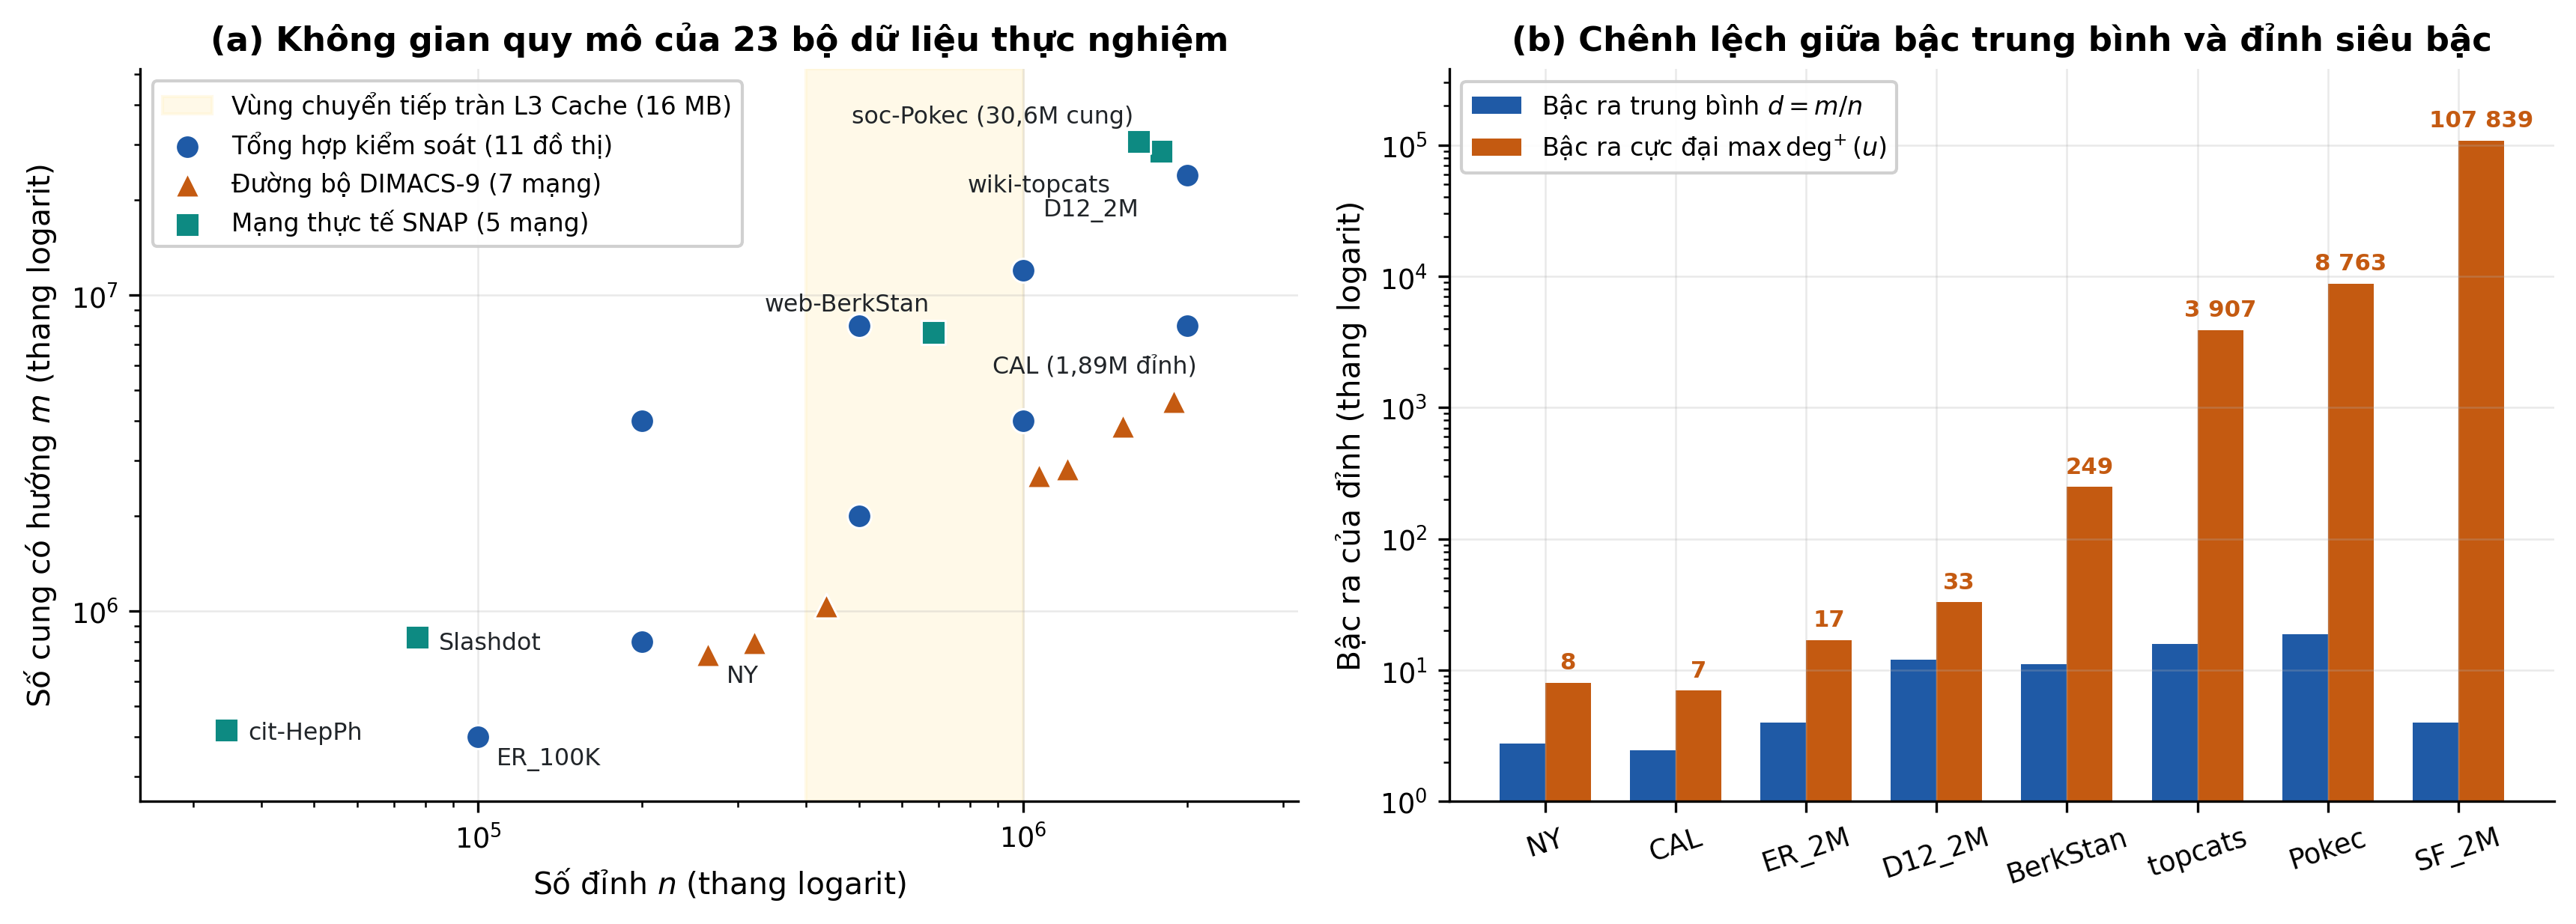
\includegraphics[width=0.96\linewidth]{image/ch3_dataset_landscape.png}
\caption{Không gian quy mô $(n, m)$ của 23 bộ dữ liệu khảo sát và sự chênh lệch giữa bậc trung bình với bậc ra cực đại.}
\label{fig:dataset_landscape}
\end{figure}

% ============================================================
% 3.3. ĐÁNH GIÁ HIỆU NĂNG TRÊN ĐỒ THỊ TỔNG HỢP KIỂM SOÁT BIẾN SỐ
% ============================================================
\section{Đánh giá hiệu năng trên đồ thị tổng hợp kiểm soát biến số}\label{sec:c3-synthetic}

Thực nghiệm trên tập đồ thị tổng hợp cho phép tách bạch rõ tác động của quy mô bộ nhớ làm việc, sự chênh lệch bậc đỉnh và mật độ cạnh lên hiệu năng đa luồng. Cụ thể, Mục~\ref{subsec:c3-syn-time} đối sánh trực tiếp thời gian giải của hệ thống với thuật toán Dijkstra tuần tự qua các mốc quy mô, sau đó Mục~\ref{subsec:c3-syn-scale} phân tích đường cong mở rộng nội tại theo số luồng và khả năng chịu tải trước các đỉnh siêu bậc.

\subsection{Thời gian giải đối sánh với Dijkstra tuần tự}\label{subsec:c3-syn-time}

Bảng~\ref{tab:syn_results} trình bày thời gian giải trung vị tính bằng mili giây của Dijkstra tuần tự và hệ thống BMSSP song song tại năm cấu hình luồng trên toàn bộ $11$ đồ thị tổng hợp. Tại quy mô nhỏ nhất \texttt{ER\_100K} với $100\,000$ đỉnh và $400\,713$ cung, toàn bộ mảng khoảng cách cùng hàng đợi nhị phân của Dijkstra nằm gọn bên trong bộ nhớ đệm L3 $16\,\mathrm{MB}$ nên Dijkstra hoàn tất trong $48{,}45\,\mathrm{ms}$, nhanh hơn nhẹ so với cấu hình tốt nhất của BMSSP ở $4$ luồng là $53{,}95\,\mathrm{ms}$ ứng với $S_{\mathrm{abs}} = 0{,}90\times$. Ở quy mô này, khối lượng cạnh trong mỗi lát đệ quy còn khiêm tốn nên phần thời gian tiết kiệm nhờ đa luồng chưa bù đắp hết chi phí duy trì cấu trúc biên phân tầng và rào chắn đồng bộ OpenMP.

\begin{table}[!htb]
\centering
\resizebox{\textwidth}{!}{%
\begin{tabular}{@{}l l r r r r r r r r@{}}
\toprule
& & & \multicolumn{5}{c}{\textbf{BMSSP theo số luồng (ms)}} & & \\
\cmidrule(lr){4-8}
\textbf{Mã đồ thị} & \textbf{Quy mô ($n$; $d$)} & \textbf{Dijkstra} & \textbf{1} & \textbf{2} & \textbf{4} & \textbf{8} & \textbf{12} & $\boldsymbol{S_{\mathrm{abs}}}$ & $\boldsymbol{S_{\mathrm{self}}}$ \\
\midrule
\texttt{ER\_100K}  & $100\mathrm{K};\; 4$  & \textbf{48,45} & 72,57 & 65,72 & 53,95 & 55,56 & 58,51 & $0{,}90\times$ & $1{,}35\times$ \\
\texttt{ER\_200K}  & $200\mathrm{K};\; 4$  & 117,19 & 174,82 & 136,68 & 113,00 & \textbf{106,75} & 110,27 & $1{,}10\times$ & $1{,}64\times$ \\
\texttt{D20\_200K} & $200\mathrm{K};\; 20$ & 254,12 & 300,91 & 244,00 & 184,86 & \textbf{163,48} & 177,86 & $1{,}55\times$ & $1{,}84\times$ \\
\texttt{ER\_500K}  & $500\mathrm{K};\; 4$  & 366,30 & 464,15 & 363,04 & 291,13 & \textbf{263,99} & 271,69 & $1{,}39\times$ & $1{,}76\times$ \\
\texttt{D16\_500K} & $500\mathrm{K};\; 16$ & 675,38 & 813,15 & 639,32 & 494,25 & \textbf{398,62} & 414,82 & $1{,}69\times$ & $2{,}04\times$ \\
\texttt{ER\_1M}    & $1{,}0\mathrm{M};\; 4$  & 746,77 & 896,54 & 705,18 & 554,14 & 500,85 & \textbf{498,66} & $1{,}50\times$ & $1{,}80\times$ \\
\texttt{SF\_1M}    & $1{,}0\mathrm{M};\; 4$  & 732,21 & 877,15 & 693,09 & 575,17 & \textbf{517,58} & 522,90 & $1{,}41\times$ & $1{,}69\times$ \\
\texttt{D12\_1M}   & $1{,}0\mathrm{M};\; 12$ & 1\,211,13 & 1\,406,66 & 1\,043,20 & 796,17 & 665,62 & \textbf{664,68} & $1{,}82\times$ & $2{,}12\times$ \\
\texttt{ER\_2M}    & $2{,}0\mathrm{M};\; 4$  & 1\,642,68 & 1\,869,91 & 1\,466,40 & 1\,119,80 & \textbf{996,52} & 1\,011,66 & $1{,}65\times$ & $1{,}88\times$ \\
\texttt{SF\_2M}    & $2{,}0\mathrm{M};\; 4$  & 1\,685,27 & 1\,913,89 & 1\,460,71 & 1\,185,89 & \textbf{1\,043,25} & 1\,057,74 & $1{,}62\times$ & $1{,}83\times$ \\
\texttt{D12\_2M}   & $2{,}0\mathrm{M};\; 12$ & 2\,645,71 & 2\,736,98 & 2\,033,11 & 1\,584,91 & 1\,330,31 & \textbf{1\,202,72} & $2{,}20\times$ & $2{,}28\times$ \\
\bottomrule
\end{tabular}%
}
\caption{Thời gian giải trung vị tính bằng ms và các hệ số tăng tốc trên 11 đồ thị tổng hợp với sai số đối chứng bằng 0.}
\label{tab:syn_results}
\end{table}

Sự đảo chiều xuất hiện ngay từ mốc $200\,000$ đỉnh và nới rộng liên tục khi quy mô đồ thị tăng lên. Trên \texttt{ER\_200K}, cấu hình $8$ luồng rút ngắn thời gian xuống $106{,}75\,\mathrm{ms}$ so với $117{,}19\,\mathrm{ms}$ của Dijkstra, đạt $S_{\mathrm{abs}} = 1{,}10\times$; khi mật độ cạnh tăng lên $d = 20$ tại \texttt{D20\_200K}, lợi thế tốc độ vọt lên $1{,}55\times$. Đáng chú ý, từ mốc $500\,000$ đỉnh trở đi, ngay cả cấu hình chỉ sử dụng $2$ luồng của BMSSP đã bắt đầu vượt qua hoặc ngang ngửa Dijkstra tuần tự, chẳng hạn $639{,}32\,\mathrm{ms}$ so với $675{,}38\,\mathrm{ms}$ trên \texttt{D16\_500K} và $2\,033{,}11\,\mathrm{ms}$ so với $2\,645{,}71\,\mathrm{ms}$ trên \texttt{D12\_2M}. Ở quy mô một triệu và hai triệu đỉnh, vùng dữ liệu hoạt động vượt xa dung lượng bộ nhớ đệm L3 khiến các thao tác hoán đổi trên cây nhị phân của Dijkstra chịu độ trễ truy cập bộ nhớ chính rất lớn. Nhờ đó, hệ thống BMSSP song song vượt Dijkstra từ $1{,}41\times$ đến $1{,}82\times$ ở nhóm một triệu đỉnh, và đạt mức tăng tốc cao nhất $S_{\mathrm{abs}} = 2{,}20\times$ trên \texttt{D12\_2M} với $24\,002\,527$ cung khi rút ngắn thời gian giải từ $2\,645{,}71\,\mathrm{ms}$ xuống còn $1\,202{,}72\,\mathrm{ms}$.

\subsection{Khả năng mở rộng nội tại và cân bằng tải trên đỉnh siêu bậc}\label{subsec:c3-syn-scale}

Hình~\ref{fig:syn_scaling} minh họa trực quan tương quan thời gian chạy ở quy mô lớn và đường cong tự tăng tốc nội tại $S_{\mathrm{self}}(p)$ khi tăng số luồng xử lý từ $1$ lên $12$. Quan sát các cột màu xanh nhạt trên Hình~\ref{fig:syn_scaling}a cho thấy ở chế độ đơn luồng $p = 1$, bản cài đặt BMSSP chỉ chậm hơn Dijkstra tuần tự từ $3{,}4\%$ trên \texttt{D12\_2M} đến khoảng $20\%$ trên đồ thị thưa $1\mathrm{M}$--$2\mathrm{M}$ đỉnh. Khoảng cách khởi điểm một luồng rất hẹp này là tiền đề quyết định giúp thuật toán nhanh chóng vượt qua bộ giải tuần tự ngay khi kích hoạt từ $2$ đến $4$ luồng công nhân.

\begin{figure}[!htb]
\centering
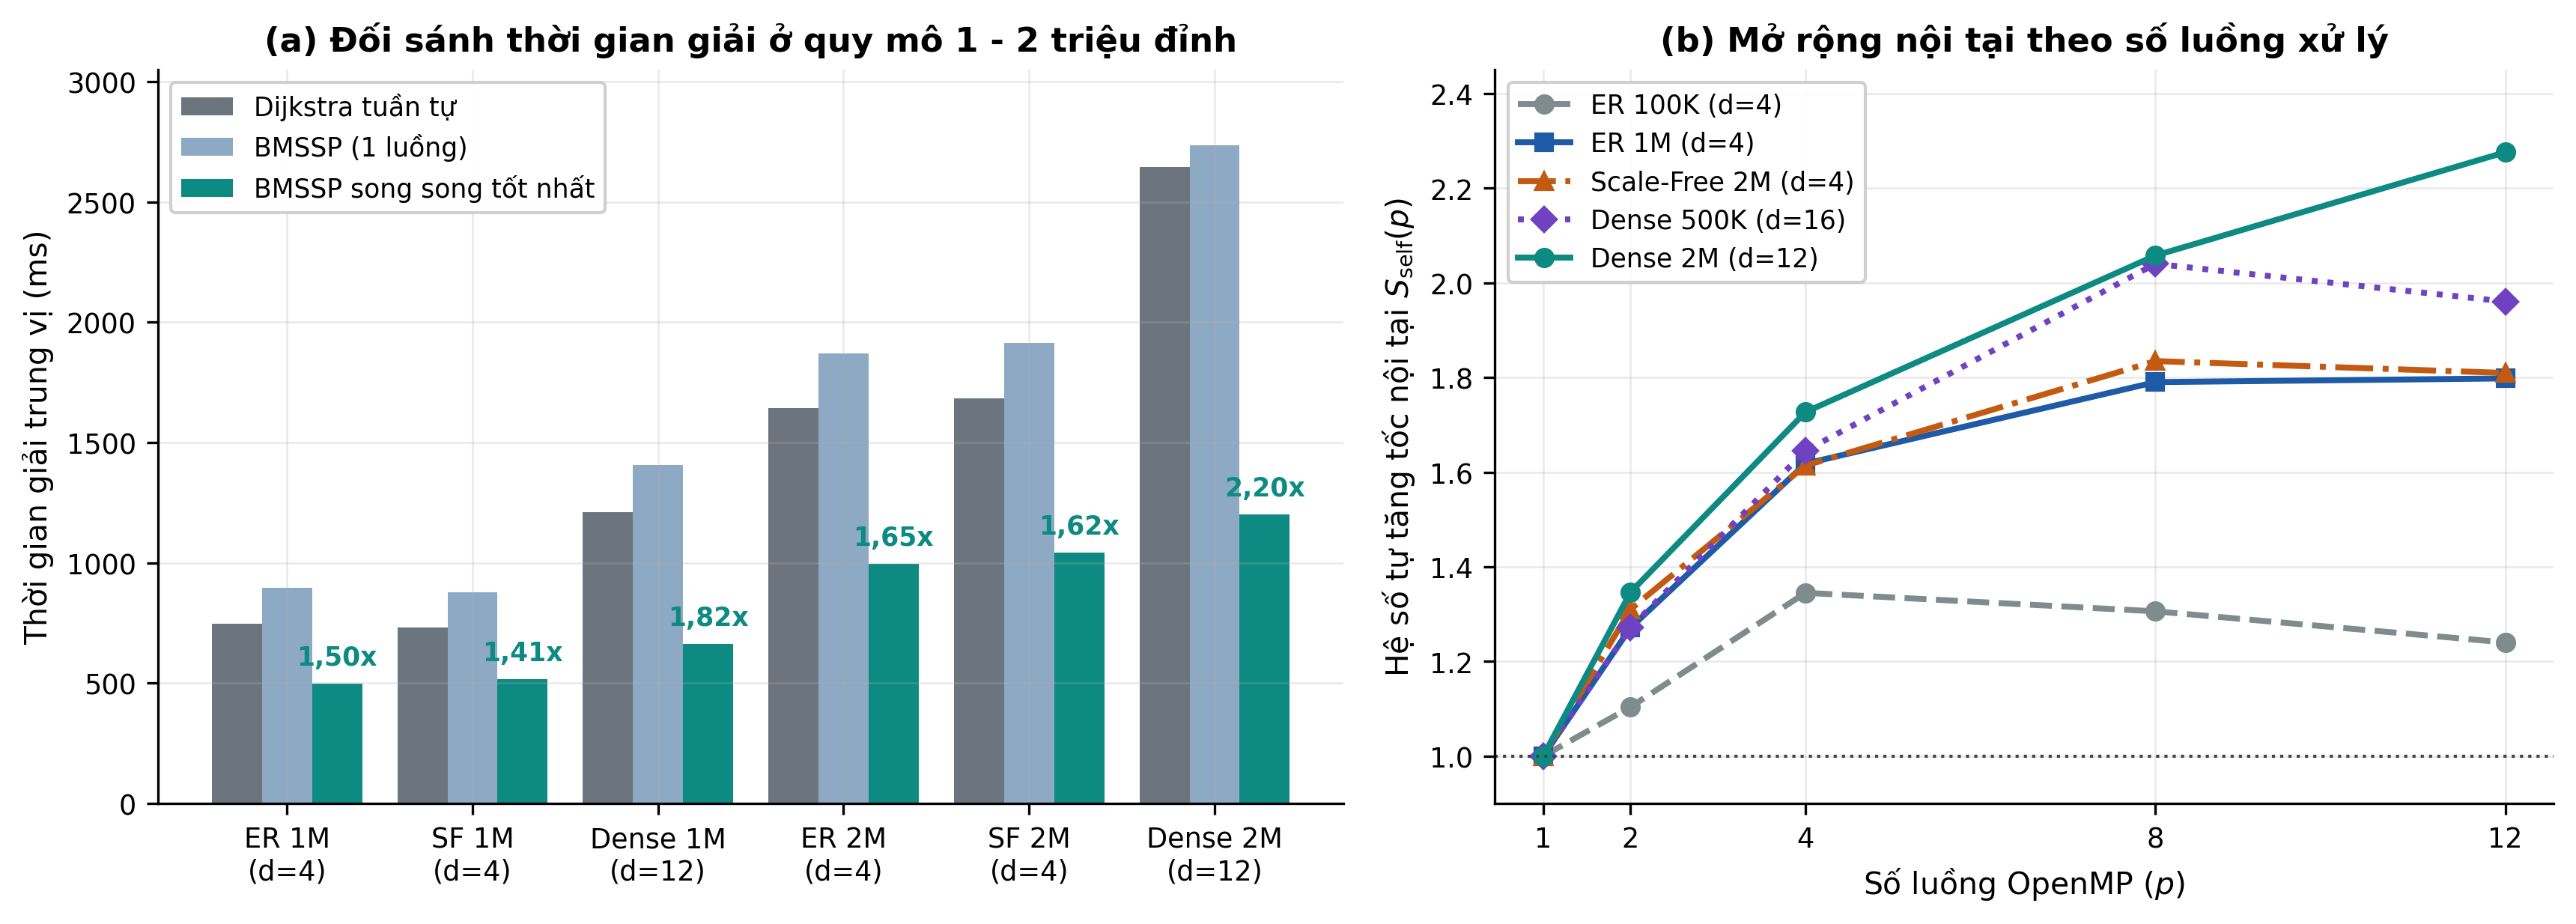
\includegraphics[width=0.96\linewidth]{image/ch3_synthetic_scaling.png}
\caption{Đối sánh thời gian giải ở quy mô 1--2 triệu đỉnh và đường cong tự tăng tốc nội tại theo số luồng trên tập đồ thị tổng hợp.}
\label{fig:syn_scaling}
\end{figure}

Về khả năng xử lý phân bố bậc lệch, phép đối sánh trên biểu đồ Hình~\ref{fig:tikz_hub_balance} giữa cặp đồ thị cùng quy mô và cùng tổng số cạnh \texttt{ER\_1M} với \texttt{SF\_1M}, cũng như \texttt{ER\_2M} với \texttt{SF\_2M}, khẳng định tính hiệu quả của chiến lược phân hoạch cạnh dựa trên mảng tổng tiền tố bậc ra và tìm kiếm nhị phân tại Mục~\ref{subsec:c2-find-pivots}. Mặc dù \texttt{SF\_2M} chứa đỉnh siêu bậc có tới $107\,839$ cung đi ra so với mức tối đa chỉ $17$ cung ở \texttt{ER\_2M}, thời gian giải tốt nhất ở $8$ luồng chỉ chênh lệch $4{,}7\%$, tương ứng $1\,043{,}25\,\mathrm{ms}$ so với $996{,}52\,\mathrm{ms}$, hoàn toàn không xảy ra hiện tượng một luồng đơn lẻ bị kẹt tại đỉnh trung tâm làm đình trệ rào chắn cuối pha.

\begin{figure}[!htb]
\centering
\resizebox{0.96\textwidth}{!}{%
\begin{tikzpicture}[>=latex, font=\scriptsize]
    % Chú giải màu phía trên
    \fill[gray!70!black] (0.2, 5.85) rectangle (0.65, 6.10);
    \node[anchor=west] at (0.75, 5.97) {Dijkstra tuần tự};
    \fill[blue!35!gray!65] (3.7, 5.85) rectangle (4.15, 6.10);
    \node[anchor=west] at (4.25, 5.97) {BMSSP 1 luồng};
    \fill[teal!75!black] (7.2, 5.85) rectangle (7.65, 6.10);
    \node[anchor=west] at (7.75, 5.97) {BMSSP 8 luồng};

    % Trục và đường lưới dọc (thang 1.0 cm = 200 ms, từ 0 đến 2000 ms -> 0 đến 10.0 cm)
    \foreach \v/\lbl in {0/0, 2.5/500, 5.0/1\,000, 7.5/1\,500, 10.0/2\,000} {
        \draw[gray!28, thin] (\v, 0.25) -- (\v, 5.55);
        \draw[black!70] (\v, 0.25) -- (\v, 0.15);
        \node[anchor=north] at (\v, 0.12) {\lbl};
    }
    \draw[->, thick, black!80] (0, 0.25) -- (10.85, 0.25);
    \draw[thick, black!80] (0, 0.25) -- (0, 5.55);
    \node[anchor=north, font=\scriptsize\bfseries] at (5.2, -0.32) {Thời gian giải trung vị (ms)};

    % Nhóm 1: ER_1M (y trung tâm = 4.90)
    \node[anchor=east, align=right, text width=3.3cm] at (-0.18, 4.90) {\textbf{\texttt{ER\_1M}} ($1\mathrm{M}$ đỉnh)\\Bậc tối đa: $17$};
    \fill[gray!70!black]   (0, 5.10) rectangle (3.734, 5.34); \node[anchor=west] at (3.82, 5.22) {746,8};
    \fill[blue!35!gray!65] (0, 4.78) rectangle (4.483, 5.02); \node[anchor=west] at (4.57, 4.90) {896,5};
    \fill[teal!75!black]   (0, 4.46) rectangle (2.504, 4.70); \node[anchor=west, text=teal!65!black, font=\scriptsize\bfseries] at (2.59, 4.58) {500,9 ms ($1{,}49\times$)};

    % Nhóm 2: SF_1M (y trung tâm = 3.60)
    \node[anchor=east, align=right, text width=3.3cm] at (-0.18, 3.60) {\textbf{\texttt{SF\_1M}} ($1\mathrm{M}$ đỉnh)\\Bậc tối đa: $62\,550$};
    \fill[gray!70!black]   (0, 3.80) rectangle (3.661, 4.04); \node[anchor=west] at (3.75, 3.92) {732,2};
    \fill[blue!35!gray!65] (0, 3.48) rectangle (4.386, 3.72); \node[anchor=west] at (4.47, 3.60) {877,2};
    \fill[teal!75!black]   (0, 3.16) rectangle (2.588, 3.40); \node[anchor=west, text=teal!65!black, font=\scriptsize\bfseries] at (2.68, 3.28) {517,6 ms ($1{,}41\times$)};

    % Nhóm 3: ER_2M (y trung tâm = 2.30)
    \node[anchor=east, align=right, text width=3.3cm] at (-0.18, 2.30) {\textbf{\texttt{ER\_2M}} ($2\mathrm{M}$ đỉnh)\\Bậc tối đa: $17$};
    \fill[gray!70!black]   (0, 2.50) rectangle (8.213, 2.74); \node[anchor=west] at (8.30, 2.62) {1\,642,7};
    \fill[blue!35!gray!65] (0, 2.18) rectangle (9.350, 2.42); \node[anchor=west] at (9.44, 2.30) {1\,869,9};
    \fill[teal!75!black]   (0, 1.86) rectangle (4.983, 2.10); \node[anchor=west, text=teal!65!black, font=\scriptsize\bfseries] at (5.07, 1.98) {996,5 ms ($1{,}65\times$)};

    % Nhóm 4: SF_2M (y trung tâm = 1.00)
    \node[anchor=east, align=right, text width=3.3cm] at (-0.18, 1.00) {\textbf{\texttt{SF\_2M}} ($2\mathrm{M}$ đỉnh)\\Bậc tối đa: $107\,839$};
    \fill[gray!70!black]   (0, 1.20) rectangle (8.426, 1.44); \node[anchor=west] at (8.51, 1.32) {1\,685,3};
    \fill[blue!35!gray!65] (0, 0.88) rectangle (9.569, 1.12); \node[anchor=west] at (9.65, 1.00) {1\,913,9};
    \fill[teal!75!black]   (0, 0.56) rectangle (5.216, 0.80); \node[anchor=west, text=teal!65!black, font=\scriptsize\bfseries] at (5.30, 0.68) {1\,043,2 ms ($1{,}62\times$)};
\end{tikzpicture}%
}
\caption{Đối sánh cân bằng tải giữa đồ thị đồng nhất Erd\H{o}s--R\'{e}nyi và đồ thị lệch bậc chứa đỉnh siêu bậc lên tới 107\,839 cung.}
\label{fig:tikz_hub_balance}
\end{figure}

Trên Hình~\ref{fig:syn_scaling}b, diễn biến giữa mức $8$ luồng và $12$ luồng phản ánh trung thực đặc trưng phần cứng của vi xử lý $6$ lõi vật lý sử dụng công nghệ đa luồng đồng thời SMT. Với các đồ thị thưa $d = 4$, mỗi cạnh chỉ thực hiện vài phép tính số học đơn giản đi kèm truy cập bộ nhớ rải rác nên băng thông bộ nhớ của $6$ lõi vật lý sớm bão hòa tại $8$ luồng với $S_{\mathrm{self}} \approx 1{,}80\times$--$1{,}88\times$. Ngược lại, trên đồ thị mật độ cao \texttt{D12\_2M} gồm $24$ triệu cung, các dải kề CSR dài giúp bộ nạp trước phần cứng hoạt động hiệu quả và nâng tỷ lệ tính toán trên mỗi dòng bộ nhớ đệm, cho phép $12$ luồng SMT tận dụng các chu kỳ trễ đường ống để đẩy hệ số tự tăng tốc nội tại lên mức cao nhất $S_{\mathrm{self}}(12) = 2{,}28\times$.

% ============================================================
% 3.4. ĐÁNH GIÁ HIỆU NĂNG TRÊN CÁC MẠNG THỰC TẾ
% ============================================================
\section{Đánh giá hiệu năng trên các mạng thực tế}\label{sec:c3-realworld}

Sau khi xác lập hành vi của hệ thống trên dữ liệu tổng hợp, bước kiểm định quan trọng tiếp theo là đặt thuật toán vào hai lớp mạng thực tế có cấu trúc đối lập nhau. Theo hướng đó, Mục~\ref{subsec:c3-road} khảo sát giới hạn thực thi của mô hình cắt lát khoảng cách trên $7$ mạng đường bộ phẳng bậc rất thấp, tiếp theo Mục~\ref{subsec:c3-snap} làm rõ quá trình chuyển pha và bứt phá tốc độ trên $5$ mạng liên kết thực tế bậc cao của Stanford SNAP.

\subsection{Giới hạn trên mạng đường bộ phẳng bậc thấp DIMACS-9}\label{subsec:c3-road}

Bảng~\ref{tab:road_results} và Hình~\ref{fig:dimacs_road} tổng hợp kết quả đo trên $7$ mạng giao thông đường bộ khu vực từ \texttt{NY} đến \texttt{CAL}. Khác biệt rõ rệt với tập đồ thị ngẫu nhiên ở mục trước, trên cả bảy mạng đường bộ có bậc ra trung bình nằm trong khoảng $2{,}34$ đến $2{,}76$, thuật toán Dijkstra tuần tự luôn duy trì thời gian giải thấp hơn. Ở cấu hình đa luồng tốt nhất từ $8$ đến $12$ luồng, thời gian của BMSSP gấp từ $1{,}70$ đến $2{,}67$ lần thời gian của Dijkstra, trong khi hệ số tự tăng tốc nội tại $S_{\mathrm{self}}$ chỉ đạt mức khiêm tốn từ $1{,}07\times$ đến $1{,}23\times$.

\begin{table}[!htb]
\centering
\resizebox{\textwidth}{!}{%
\begin{tabular}{@{}l l r r r r r r r r r@{}}
\toprule
& & & & & \multicolumn{4}{c}{\textbf{BMSSP theo số luồng (ms)}} & & \\
\cmidrule(lr){6-9}
\textbf{Mã} & \textbf{Khu vực} & \textbf{Số đỉnh $n$} & \textbf{Số cung $m$} & \textbf{Dijkstra} & \textbf{1} & \textbf{4} & \textbf{8} & \textbf{12} & $\boldsymbol{T_{\mathrm{par}}/T_{\mathrm{base}}}$ & $\boldsymbol{S_{\mathrm{self}}}$ \\
\midrule
\texttt{NY}  & New York       & 264\,346    & 730\,100    & \textbf{63,71}  & 201,77 & 178,68 & 174,09 & 166,87 & $2{,}62\times$ & $1{,}21\times$ \\
\texttt{BAY} & Vịnh SF        & 321\,270    & 794\,830    & \textbf{73,20}  & 223,30 & 203,55 & 195,39 & 196,59 & $2{,}67\times$ & $1{,}14\times$ \\
\texttt{COL} & Colorado       & 435\,666    & 1\,042\,400 & \textbf{101,79} & 269,06 & 238,61 & 241,02 & 236,77 & $2{,}33\times$ & $1{,}14\times$ \\
\texttt{FLA} & Florida        & 1\,070\,376 & 2\,687\,902 & \textbf{226,74} & 638,99 & 577,49 & 541,95 & 563,35 & $2{,}39\times$ & $1{,}18\times$ \\
\texttt{NW}  & Tây Bắc Mỹ     & 1\,207\,945 & 2\,820\,776 & \textbf{295,80} & 659,74 & 616,08 & 614,24 & 615,09 & $2{,}08\times$ & $1{,}07\times$ \\
\texttt{NE}  & Đông Bắc Mỹ    & 1\,524\,453 & 3\,857\,376 & \textbf{445,99} & 936,50 & 803,36 & 758,88 & 760,91 & $1{,}70\times$ & $1{,}23\times$ \\
\texttt{CAL} & California--NV & 1\,890\,815 & 4\,620\,230 & \textbf{482,93} & 1\,077,89 & 985,64 & 914,01 & 891,43 & $1{,}85\times$ & $1{,}21\times$ \\
\bottomrule
\end{tabular}%
}
\caption{Thời gian giải trung vị tính bằng ms và tỷ số tốc độ trên 7 mạng đường bộ Hoa Kỳ thuộc bộ chuẩn DIMACS-9.}
\label{tab:road_results}
\end{table}

Hiện tượng này bắt nguồn trực tiếp từ sự tương tác giữa cấu trúc hình học phẳng hai chiều với hai giới hạn phần cứng đã phân tích tại Bảng~\ref{tab:theory_vs_hardware} của Chương~\ref{chap:parallel_bmssp}. Thứ nhất, mặt sóng lan truyền khoảng cách trên mạng giao lộ phẳng chỉ là một vành đai địa lý mỏng gồm vài chục đến vài trăm đỉnh ở mỗi thời điểm; cộng thêm bậc ra trung bình chỉ khoảng $2{,}5$, tổng số cung hoạt động $N_{\mathrm{act}}$ trong phần lớn các bước lặp của \textsc{FindPivots} và các lời gọi đệ quy tầng sâu đều rơi xuống dưới ngưỡng độ hạt $\Theta_{\mathrm{cutoff}} = 2048$. Hệ quả là phần lớn quá trình giải tự động chuyển về thực thi tuần tự trong khi vẫn phải gánh chi phí phân tách đệ quy nhiều tầng và quản lý cấu trúc biên $\mathcal{D}$. Thứ hai, các giao lộ gần nhau ngoài thực địa trong dữ liệu đường bộ thường có mã chỉ số đỉnh nằm sát nhau trên mảng bộ nhớ, đồng thời kích thước hàng đợi ưu tiên của Dijkstra trên đồ thị phẳng luôn rất nhỏ so với tổng số đỉnh. Nhờ tính cục bộ không gian cao đó, Dijkstra giải xong mạng \texttt{FLA} $1{,}07\mathrm{M}$ đỉnh chỉ trong $226{,}74\,\mathrm{ms}$, nhanh hơn gấp ba lần so với chính Dijkstra trên đồ thị ngẫu nhiên \texttt{ER\_1M} có cùng số đỉnh là $746{,}77\,\mathrm{ms}$.

\begin{figure}[!htb]
\centering
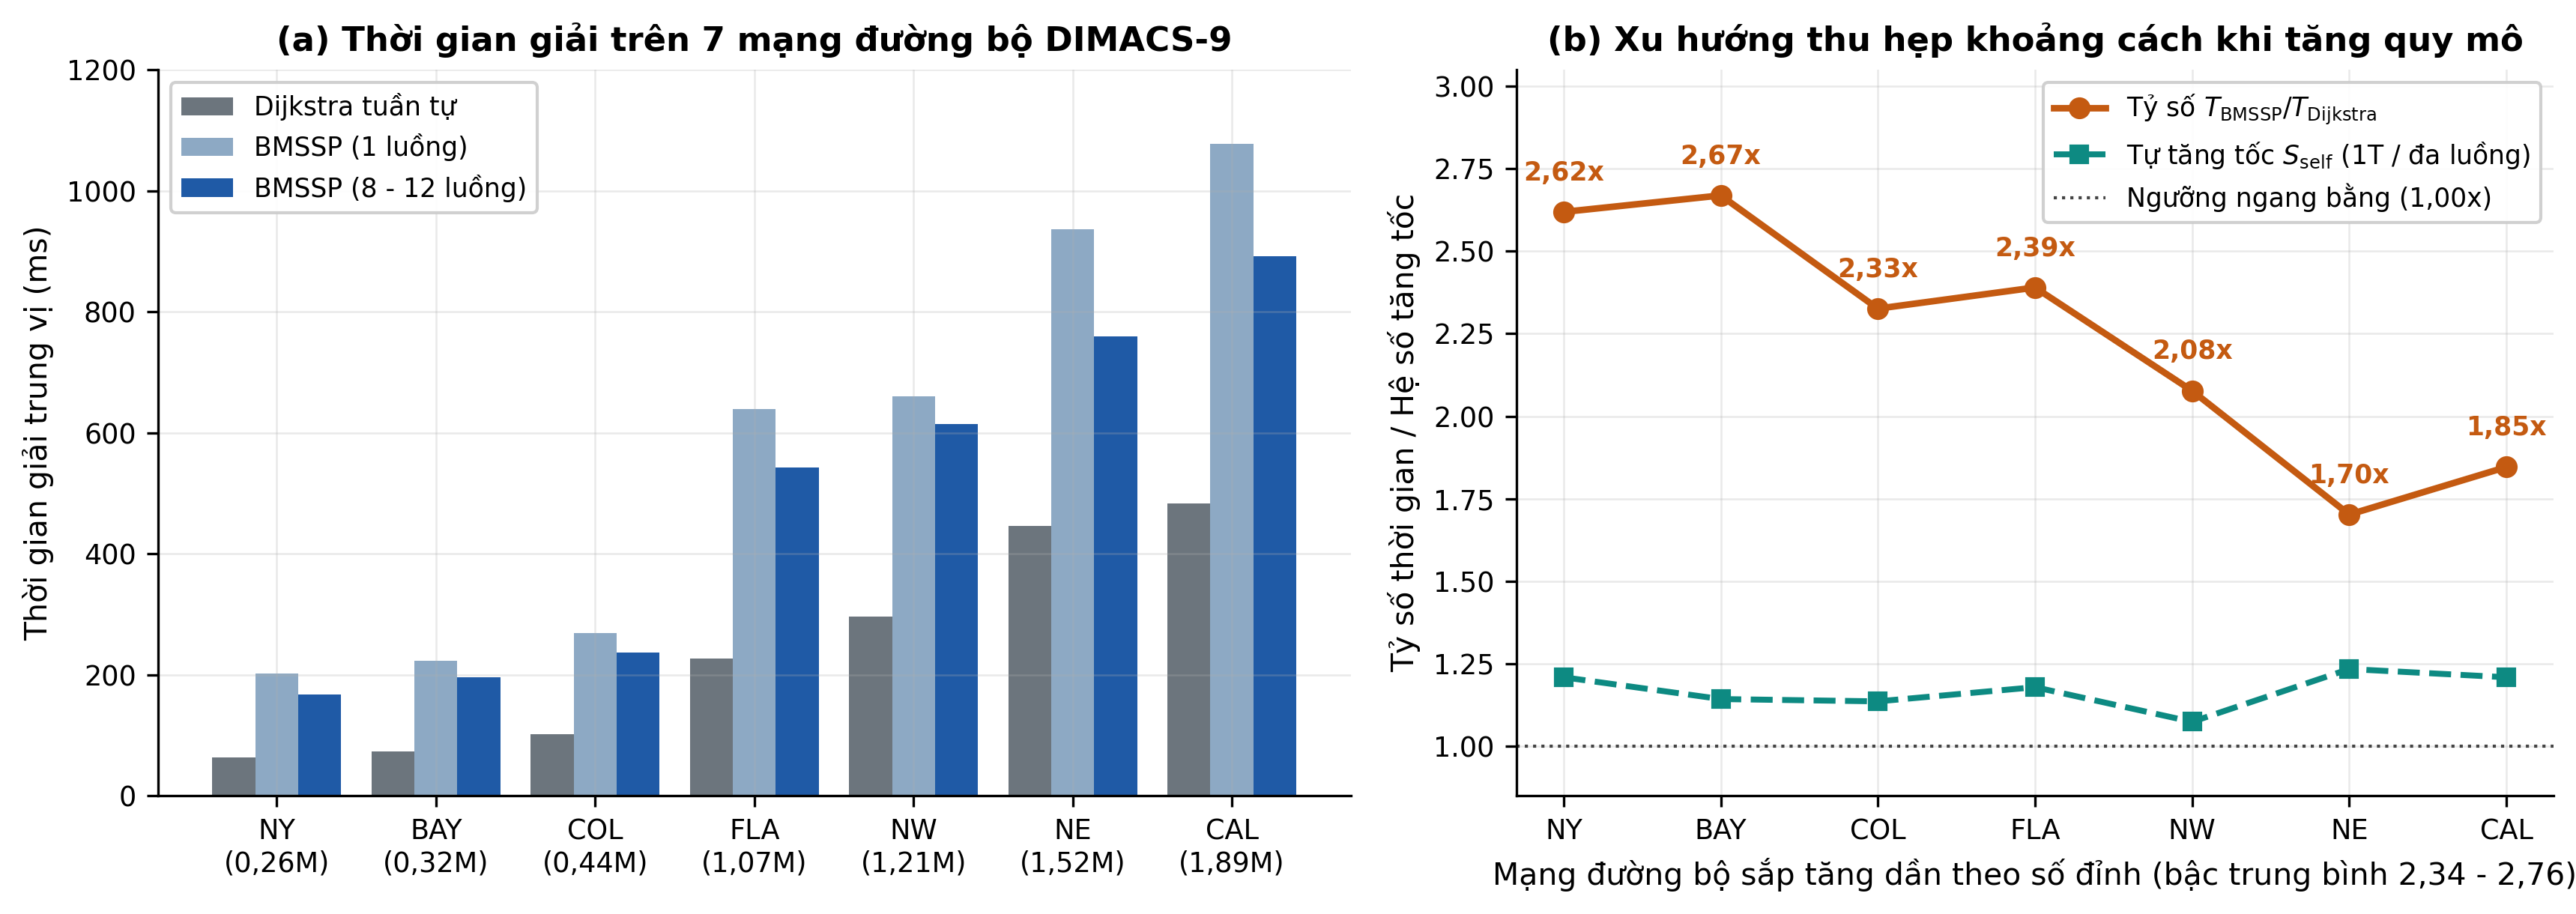
\includegraphics[width=0.96\linewidth]{image/ch3_dimacs_road.png}
\caption{Thời gian giải và xu hướng giảm dần tỷ số $T_{\mathrm{BMSSP}} / T_{\mathrm{Dijkstra}}$ khi quy mô đỉnh tăng trên 7 mạng đường bộ DIMACS-9.}
\label{fig:dimacs_road}
\end{figure}

Mặc dù chưa vượt qua Dijkstra ở dải bậc cực thấp này, đường màu cam trên Hình~\ref{fig:dimacs_road}b vẫn bộc lộ một xu hướng hội tụ nhất quán theo quy mô đỉnh. Khi kích thước mạng tăng gấp sáu lần từ \texttt{BAY} với $0{,}32\mathrm{M}$ đỉnh lên hành lang đô thị Đông Bắc \texttt{NE} với $1{,}52\mathrm{M}$ đỉnh và \texttt{CAL} với $1{,}89\mathrm{M}$ đỉnh, vành đai mặt sóng mở rộng hơn giúp hệ số tự tăng tốc nội tại nhích lên $1{,}21\times$--$1{,}23\times$, đồng thời mảng trạng thái vượt quá bộ nhớ đệm L3 làm giảm lợi thế cục bộ của Dijkstra. Qua đó, tỷ số thời gian $T_{\mathrm{BMSSP}} / T_{\mathrm{Dijkstra}}$ thu hẹp đều đặn từ mức $2{,}67\times$ ở \texttt{BAY} xuống $2{,}33\times$ ở \texttt{COL}, $2{,}08\times$ ở \texttt{NW} và chỉ còn $1{,}70\times$--$1{,}85\times$ tại \texttt{NE} và \texttt{CAL}.

\subsection{Điểm đảo chiều và ưu thế trên mạng thực tế bậc cao Stanford SNAP}\label{subsec:c3-snap}

Khi chuyển từ mạng giao thông phẳng sang các mạng thông tin và xã hội thực tế có bậc trung bình từ $10{,}71$ đến $18{,}75$ trong Bảng~\ref{tab:snap_results}, bức tranh hiệu năng thay đổi căn bản và tái hiện rõ nét một đường cong chuyển pha đơn điệu theo quy mô đỉnh như thể hiện trên Hình~\ref{fig:snap_highdeg} và Hình~\ref{fig:tikz_snap_bars}.

\begin{table}[!htb]
\centering
\resizebox{\textwidth}{!}{%
\begin{tabular}{@{}l r r r r r r r r r r@{}}
\toprule
& & & & \multicolumn{5}{c}{\textbf{BMSSP theo số luồng (ms)}} & & \\
\cmidrule(lr){5-9}
\textbf{Bộ dữ liệu} & \textbf{Số đỉnh $n$} & \textbf{Bậc $d$} & \textbf{Dijkstra} & \textbf{1} & \textbf{2} & \textbf{4} & \textbf{8} & \textbf{12} & $\boldsymbol{S_{\mathrm{abs}}}$ & $\boldsymbol{S_{\mathrm{self}}}$ \\
\midrule
\texttt{cit-HepPh}        & 34\,546     & 12,20 & \textbf{6,41}  & 19,10 & 19,75 & 18,20 & 21,20 & 19,50 & $0{,}35\times$ & $1{,}05\times$ \\
\texttt{soc-Slashdot0811} & 77\,360     & 10,71 & \textbf{53,06} & 72,95 & 80,62 & 73,23 & 66,20 & 64,86 & $0{,}82\times$ & $1{,}12\times$ \\
\texttt{web-BerkStan}     & 685\,230    & 11,09 & 299,01 & 464,93 & 447,04 & 403,07 & \textbf{291,25} & 299,11 & $1{,}03\times$ & $1{,}60\times$ \\
\texttt{wiki-topcats}     & 1\,791\,489 & 15,91 & 2\,219,93 & 2\,535,15 & 1\,906,69 & 1\,421,54 & 1\,336,99 & \textbf{1\,315,10} & $1{,}69\times$ & $1{,}93\times$ \\
\texttt{soc-Pokec}        & 1\,632\,803 & 18,75 & 2\,474,98 & 2\,520,72 & 1\,859,25 & 1\,442,74 & 1\,462,64 & \textbf{1\,351,73} & $1{,}83\times$ & $1{,}86\times$ \\
\bottomrule
\end{tabular}%
}
\caption{Thời gian giải trung vị tính bằng ms và hệ số tăng tốc trên 5 mạng thực tế bậc cao từ kho dữ liệu Stanford SNAP.}
\label{tab:snap_results}
\end{table}

Ở hai mạng quy mô nhỏ dưới $100\,000$ đỉnh, dữ liệu nằm trọn trong bộ nhớ đệm tốc độ cao của vi xử lý. Trên mạng trích dẫn có hướng không chu trình \texttt{cit-HepPh}, nguồn chỉ đi tới $20\,507$ đỉnh nên Dijkstra kết thúc sau $6{,}41\,\mathrm{ms}$, trong khi BMSSP mất $18{,}20\,\mathrm{ms}$ ứng với $S_{\mathrm{abs}} = 0{,}35\times$ do chi phí cố định khởi tạo vùng làm việc cho các tầng đệ quy. Tuy nhiên, ngay khi quy mô tăng lên $77\,360$ đỉnh liên thông toàn phần trên mạng cộng đồng \texttt{soc-Slashdot0811}, thời gian của Dijkstra tăng vọt hơn tám lần lên $53{,}06\,\mathrm{ms}$, còn BMSSP chỉ tăng lên $64{,}86\,\mathrm{ms}$, kéo hệ số $S_{\mathrm{abs}}$ tiến sát ngưỡng cân bằng ở mức $0{,}82\times$.

\begin{figure}[!htb]
\centering
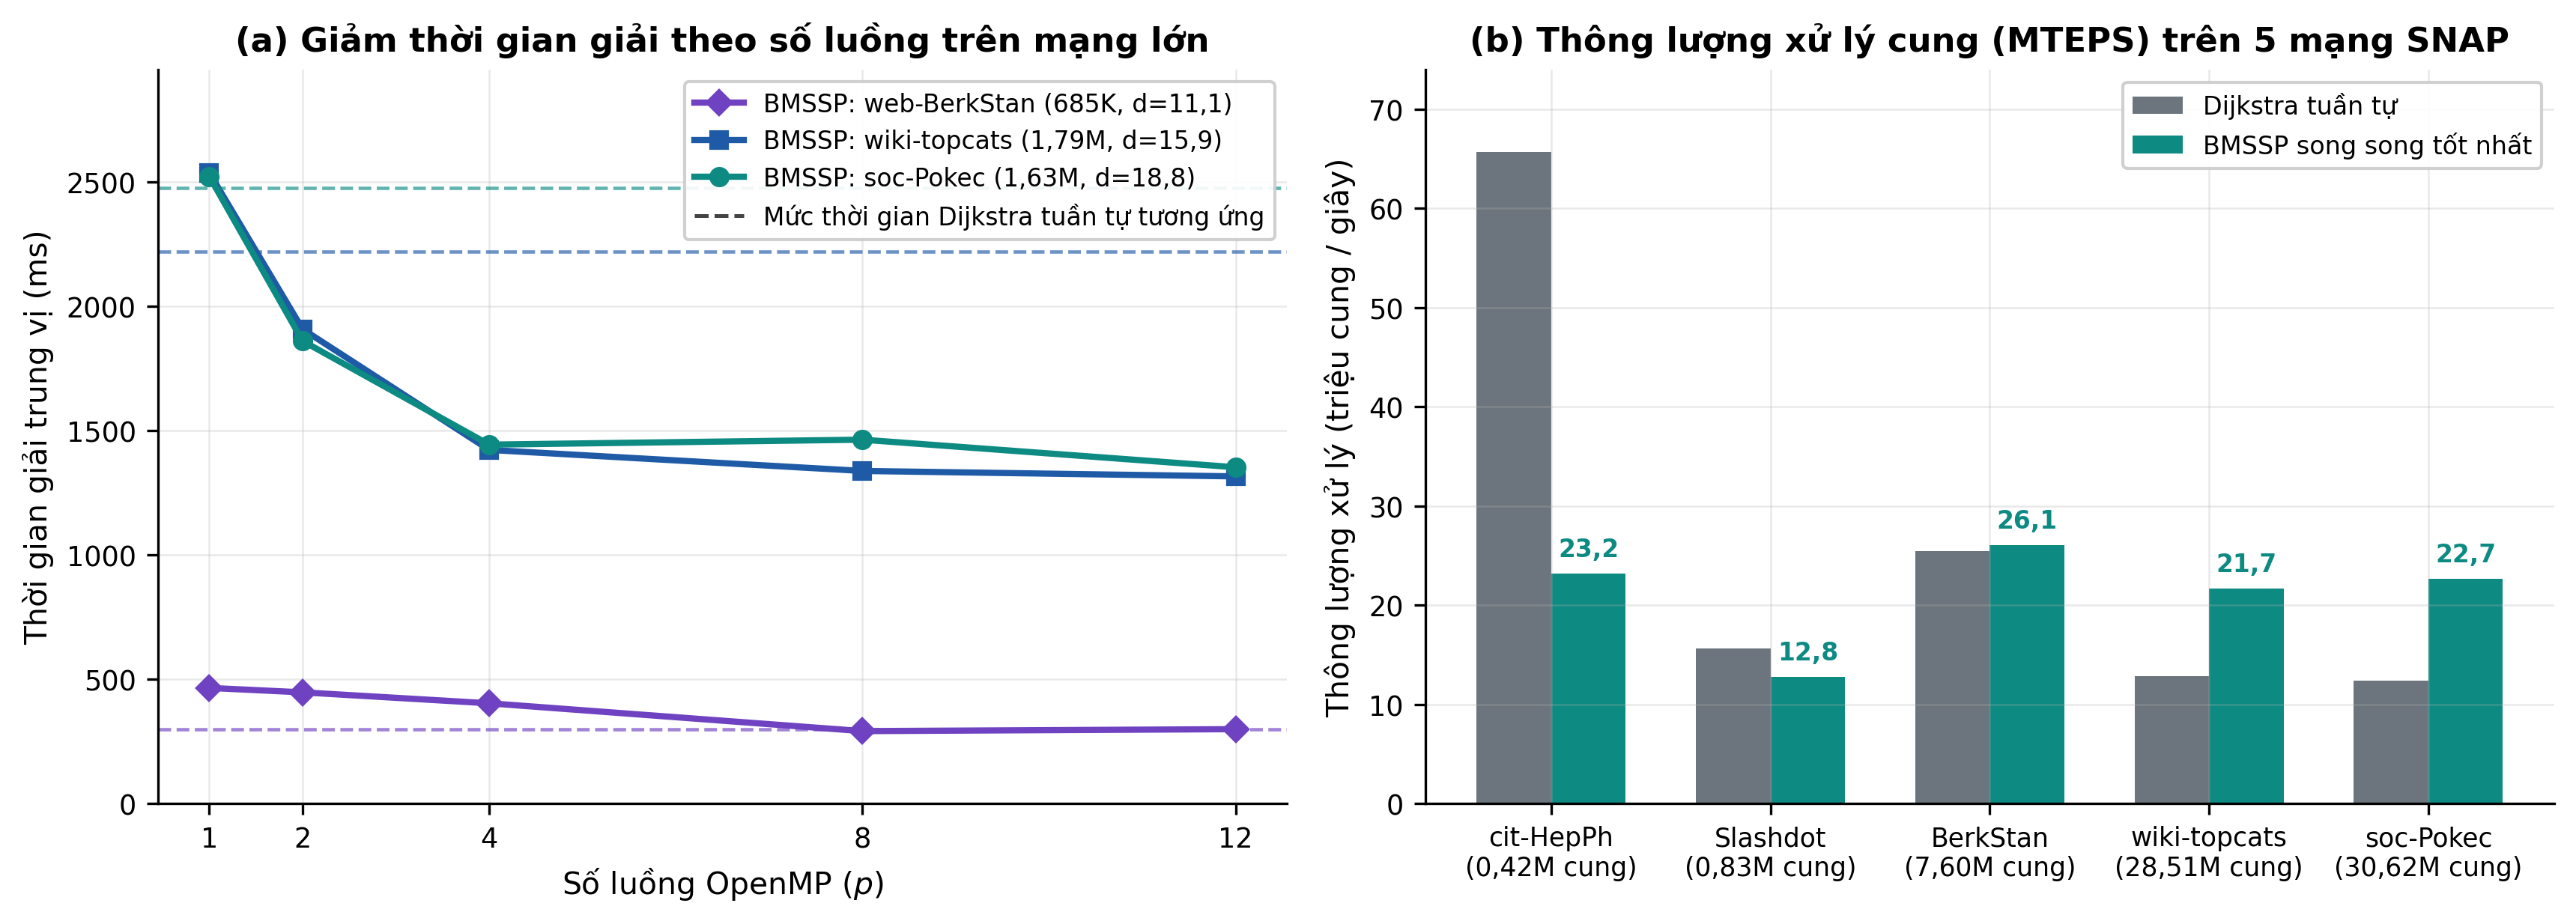
\includegraphics[width=0.96\linewidth]{image/ch3_snap_highdeg.png}
\caption{Đường cong giảm thời gian giải theo số luồng và thông lượng xử lý triệu cung mỗi giây trên 5 mạng thực tế Stanford SNAP.}
\label{fig:snap_highdeg}
\end{figure}

Điểm cắt thực nghiệm trên dữ liệu thực tế xuất hiện tại mạng liên kết Web \texttt{web-BerkStan} gồm $685\,230$ đỉnh và $7\,600\,595$ cung, trong đó có $459\,831$ đỉnh tới được từ nguồn. Dù các trang Web thuộc cùng hệ thống tên miền có tính phân cụm cục bộ rất cao tạo thuận lợi cho bộ nhớ đệm của Dijkstra, khối lượng cạnh trên mỗi lát của \texttt{web-BerkStan} đã đủ lớn để kích hoạt hiệu quả vùng công nhân OpenMP với $S_{\mathrm{self}}(8) = 1{,}60\times$, giúp BMSSP ở $8$ luồng đạt $291{,}25\,\mathrm{ms}$ và chính thức vượt nhẹ Dijkstra tuần tự ở mức $299{,}01\,\mathrm{ms}$ tương ứng $S_{\mathrm{abs}} = 1{,}03\times$.

\begin{figure}[!htb]
\centering
\resizebox{0.94\textwidth}{!}{%
\begin{tikzpicture}[>=latex, font=\scriptsize]
    % Chú giải phía trên (đồng bộ 1-1 với toàn bộ màu trên biểu đồ)
    \fill[teal!75!black] (1.10, 5.72) rectangle (1.60, 5.97);
    \node[anchor=west] at (1.72, 5.85) {Tăng tốc so với Dijkstra $S_{\mathrm{abs}}$};
    \fill[blue!42!gray!70] (5.95, 5.72) rectangle (6.45, 5.97);
    \node[anchor=west] at (6.57, 5.85) {Tự tăng tốc nội tại $S_{\mathrm{self}}$};
    \draw[red!70!black, dashed, very thick] (10.25, 5.85) -- (10.95, 5.85);
    \node[anchor=west, text=red!70!black] at (11.07, 5.85) {Ngưỡng cân bằng $1{,}00\times$};

    % Lưới ngang (thang 1,00x = 2,60 cm -> 2,00x = 5,20 cm)
    \foreach \yv/\ylbl in {0.0/0{,}00, 1.30/0{,}50, 2.60/1{,}00, 3.90/1{,}50, 5.20/2{,}00} {
        \draw[gray!26, thin] (0.40, \yv) -- (13.95, \yv);
        \draw[black!70] (0.40, \yv) -- (0.30, \yv);
        \node[anchor=east] at (0.26, \yv) {$\ylbl\times$};
    }
    \draw[->, thick, black!80] (0.40, 0) -- (14.20, 0);
    \draw[->, thick, black!80] (0.40, 0) -- (0.40, 5.55);
    \node[rotate=90, anchor=south, font=\scriptsize\bfseries] at (-0.68, 2.75) {Hệ số tăng tốc};

    % Đường ngưỡng cân bằng 1,00x
    \draw[red!70!black, dashed, very thick] (0.40, 2.60) -- (13.95, 2.60);

    % Cụm 1: cit-HepPh (xc = 1.85)
    \fill[teal!75!black]   (1.13, 0) rectangle (1.77, 0.91);
    \fill[blue!42!gray!70] (1.93, 0) rectangle (2.57, 2.73);
    \node[anchor=south, font=\scriptsize\bfseries, text=teal!65!black] at (1.45, 0.94) {$0{,}35\times$};
    \node[anchor=south, text=blue!50!black] at (2.25, 2.76) {$1{,}05\times$};
    \node[anchor=north, align=center] at (1.85, -0.10) {\texttt{cit-HepPh}\\($34{,}5\mathrm{K}$)};

    % Cụm 2: Slashdot0811 (xc = 4.55)
    \fill[teal!75!black]   (3.83, 0) rectangle (4.47, 2.13);
    \fill[blue!42!gray!70] (4.63, 0) rectangle (5.27, 2.91);
    \node[anchor=south, font=\scriptsize\bfseries, text=teal!65!black] at (4.15, 2.15) {$0{,}82\times$};
    \node[anchor=south, text=blue!50!black] at (4.95, 2.94) {$1{,}12\times$};
    \node[anchor=north, align=center] at (4.55, -0.10) {\texttt{Slashdot0811}\\($77{,}4\mathrm{K}$)};

    % Cụm 3: web-BerkStan (xc = 7.25)
    \fill[teal!75!black]   (6.53, 0) rectangle (7.17, 2.68);
    \fill[blue!42!gray!70] (7.33, 0) rectangle (7.97, 4.16);
    \node[anchor=south, font=\scriptsize\bfseries, text=teal!65!black] at (6.85, 2.71) {$1{,}03\times$};
    \node[anchor=south, text=blue!50!black] at (7.65, 4.19) {$1{,}60\times$};
    \node[anchor=north, align=center] at (7.25, -0.10) {\texttt{web-BerkStan}\\($685\mathrm{K}$)};

    % Cụm 4: wiki-topcats (xc = 9.95)
    \fill[teal!75!black]   (9.23, 0) rectangle (9.87, 4.39);
    \fill[blue!42!gray!70] (10.03, 0) rectangle (10.67, 5.02);
    \node[anchor=south, font=\scriptsize\bfseries, text=teal!65!black] at (9.55, 4.42) {$1{,}69\times$};
    \node[anchor=south, text=blue!50!black] at (10.35, 5.05) {$1{,}93\times$};
    \node[anchor=north, align=center] at (9.95, -0.10) {\texttt{wiki-topcats}\\($1{,}79\mathrm{M}$)};

    % Cụm 5: soc-Pokec (xc = 12.65)
    \fill[teal!75!black]   (11.93, 0) rectangle (12.57, 4.76);
    \fill[blue!42!gray!70] (12.73, 0) rectangle (13.37, 4.84);
    \node[anchor=south, font=\scriptsize\bfseries, text=teal!65!black] at (12.25, 4.79) {$1{,}83\times$};
    \node[anchor=south, text=blue!50!black] at (13.05, 4.87) {$1{,}86\times$};
    \node[anchor=north, align=center] at (12.65, -0.10) {\texttt{soc-Pokec}\\($1{,}63\mathrm{M}$)};
\end{tikzpicture}%
}
\caption{Quá trình chuyển pha đơn điệu của hệ số tăng tốc $S_{\mathrm{abs}}$ và $S_{\mathrm{self}}$ theo quy mô tăng dần trên 5 mạng thực tế SNAP.}
\label{fig:tikz_snap_bars}
\end{figure}

Khi tiến vào vùng quy mô trên $1{,}6$ triệu đỉnh và xấp xỉ $30$ triệu cung của hai mạng \texttt{wiki-topcats} và \texttt{soc-Pokec}, ưu thế của kiến trúc BMSSP song song thể hiện toàn diện trên cả thời gian thực thi lẫn thông lượng xử lý cung trên Hình~\ref{fig:snap_highdeg}b. Ngay ở cấu hình một luồng, thời gian của BMSSP trên \texttt{soc-Pokec} là $2\,520{,}72\,\mathrm{ms}$, xấp xỉ ngang bằng mức $2\,474{,}98\,\mathrm{ms}$ của Dijkstra. Khi mở rộng lên $12$ luồng, thời gian giải giảm mạnh xuống còn $1\,315{,}10\,\mathrm{ms}$ trên \texttt{wiki-topcats} ứng với thông lượng $21{,}7$ triệu cung mỗi giây và $1\,351{,}73\,\mathrm{ms}$ trên \texttt{soc-Pokec} ứng với $22{,}7$ triệu cung mỗi giây, vượt xa mức thông lượng bị suy giảm còn khoảng $12{,}4$--$12{,}8$ triệu cung mỗi giây của Dijkstra tuần tự. Kết quả là hệ thống giải nhanh hơn Dijkstra lần lượt $1{,}69\times$ và $1{,}83\times$, tiết kiệm hơn $0{,}90$ đến $1{,}12$ giây cho mỗi truy vấn đường đi ngắn nhất.

% ============================================================
% 3.5. PHÂN TÍCH TỔNG HỢP QUY LUẬT (N, D) VÀ NÚT THẮT HỆ THỐNG
% ============================================================
\section{Phân tích tổng hợp mối liên hệ giữa quy mô đỉnh, bậc đỉnh và nút thắt hệ thống}\label{sec:c3-tong-hop}

Kết hợp toàn bộ $23$ phép đo từ ba nhóm dữ liệu cho phép giải thích thống nhất vì sao cùng một kiến trúc BMSSP song song lại chậm hơn trên mạng đường bộ nhưng vượt xa Dijkstra trên mạng xã hội và đồ thị bậc cao. Để làm sáng tỏ bản chất này, Mục~\ref{subsec:c3-co-che} phân tích cơ chế phân tách chi phí theo bậc đỉnh gắn liền với hiệu suất luồng và các nút thắt nội tại của hệ thống, sau đó Mục~\ref{subsec:c3-phase-law} xây dựng bản đồ phân vùng ưu thế trên mặt phẳng $(n, d)$ cùng bảng hướng dẫn lựa chọn thuật toán thực tiễn.

\subsection{Cơ chế phân tách chi phí theo bậc đỉnh và các nút thắt nội tại}\label{subsec:c3-co-che}

Sự khác biệt cốt lõi giữa hai thuật toán nằm ở cách thời gian thực thi phản ứng khi mật độ cạnh $d = m/n$ tăng lên trên cùng một quy mô đỉnh $n$. Đối với Dijkstra tuần tự, thời gian giải thực nghiệm tuân theo cấu trúc chi phí gồm hai thành phần gắn chặt trên một luồng duy nhất:
\begin{equation}
    T_{\mathrm{Dijkstra}}(n, d) \approx c_{\mathrm{heap}}(n)\,n\log_2 n + c_{\mathrm{relax}}(n)\,n d,
    \label{eq:emp-dijkstra}
\end{equation}
trong đó hệ số $c_{\mathrm{heap}}(n)$ và $c_{\mathrm{relax}}(n)$ tăng mạnh khi $n$ vượt ngưỡng bộ nhớ đệm L3 $16\,\mathrm{MB}$ ở khoảng $400\mathrm{K}$--$1\mathrm{M}$ đỉnh. Khi bậc $d$ tăng cao trên mạng liên kết toàn cục, hàng triệu phép cải thiện khoảng cách liên tục đẩy bản ghi mới vào cây heap nhị phân và phát sinh truy cập bộ nhớ ngẫu nhiên trên một lõi đơn. Ngược lại, từ thiết kế hai phân vùng tại Chương~\ref{chap:parallel_bmssp}, thời gian thực thi của hệ thống BMSSP song song với $p$ luồng có thể biểu diễn qua ba thành phần:
\begin{equation}
    T_{\mathrm{BMSSP}}(n, d, p) \approx T_{\mathrm{seq}}(n) + c_{\mathcal{D}}(n)\,n\log_2^{2/3} n + \frac{c_{\mathrm{CSR}}\,n d}{p_{\mathrm{eff}}(n, d)},
    \label{eq:emp-bmssp}
\end{equation}
trong đó $T_{\mathrm{seq}}(n)$ là chi phí điều phối đệ quy và các bước tuần tự cố hữu như \textsc{BaseCase}, dựng rừng đỉnh cha trong \textsc{FindPivots} và chèn tiền tố \textsc{BatchPrepend}; thành phần thứ hai đại diện cho chi phí quản lý đỉnh chờ bên trong \texttt{Concurrent\allowbreak FrontierD} bao gồm thao tác rút biên \textsc{Pull} dưới khóa rút riêng; còn thành phần thứ ba là chi phí quét các dải kề CSR liên tiếp được chia đều cho số luồng hiệu dụng $p_{\mathrm{eff}}$.

\begin{figure}[!htb]
\centering
\resizebox{0.94\textwidth}{!}{%
\begin{tikzpicture}[>=latex, font=\scriptsize]
    % Hệ trục Hiệu suất song song E(p) (%) theo p = 1, 2, 4, 8, 12
    % Trục x: p=1 -> 1.0, p=2 -> 3.3, p=4 -> 5.6, p=8 -> 7.9, p=12 -> 10.2
    % Trục y: 0% -> 0.0, 100% -> 4.40 cm (1% = 0.044 cm)
    \foreach \yp/\yl in {0/0\%, 20/20\%, 40/40\%, 60/60\%, 80/80\%, 100/100\%} {
        \pgfmathsetmacro{\yy}{\yp * 0.044}
        \draw[gray!26, thin] (0.6, \yy) -- (10.7, \yy);
        \draw[black!70] (0.6, \yy) -- (0.50, \yy);
        \node[anchor=east] at (0.45, \yy) {\yl};
    }
    \foreach \xp/\xl in {1.0/1, 3.3/2, 5.6/4, 7.9/8, 10.2/12} {
        \draw[gray!22, thin] (\xp, 0) -- (\xp, 4.55);
        \draw[black!70] (\xp, 0) -- (\xp, -0.10);
        \node[anchor=north] at (\xp, -0.14) {\xl};
    }
    \draw[->, thick, black!80] (0.6, 0) -- (11.0, 0);
    \draw[->, thick, black!80] (0.6, 0) -- (0.6, 4.75);
    \node[anchor=north, font=\scriptsize\bfseries] at (5.65, -0.52) {Số luồng OpenMP ($p$)};
    \node[rotate=90, anchor=south, font=\scriptsize\bfseries] at (-0.55, 2.30) {Hiệu suất song song $E(p) = S_{\mathrm{self}}(p)/p$};

    % Đường 1: D12_2M (100, 67.3, 43.2, 25.7, 19.0) -> y = (4.40, 2.96, 1.90, 1.13, 0.84)
    \draw[teal!75!black, very thick] (1.0,4.40) -- (3.3,2.96) -- (5.6,1.90) -- (7.9,1.13) -- (10.2,0.84);
    \foreach \x/\y in {1.0/4.40, 3.3/2.96, 5.6/1.90, 7.9/1.13, 10.2/0.84} \fill[teal!75!black] (\x,\y) circle (2.3pt);
    \node[anchor=south west, text=teal!70!black] at (3.35, 2.98) {67,3\%};
    \node[anchor=south west, text=teal!70!black] at (7.95, 1.15) {25,7\%};

    % Đường 2: soc-Pokec (100, 67.8, 43.7, 21.5, 15.5) -> y = (4.40, 2.98, 1.92, 0.95, 0.68)
    \draw[blue!65!black, very thick, dashed] (1.0,4.40) -- (3.3,2.98) -- (5.6,1.92) -- (7.9,0.95) -- (10.2,0.68);
    \foreach \x/\y in {1.0/4.40, 3.3/2.98, 5.6/1.92, 7.9/0.95, 10.2/0.68} \fill[blue!65!black] (\x-0.07,\y-0.07) rectangle (\x+0.07,\y+0.07);

    % Đường 3: web-BerkStan (100, 52.0, 28.8, 20.0, 13.0) -> y = (4.40, 2.29, 1.27, 0.88, 0.57)
    \draw[violet!75!black, thick, dashdotted] (1.0,4.40) -- (3.3,2.29) -- (5.6,1.27) -- (7.9,0.88) -- (10.2,0.57);
    \foreach \x/\y in {1.0/4.40, 3.3/2.29, 5.6/1.27, 7.9/0.88, 10.2/0.57} \fill[violet!75!black] (\x,\y) circle (2.0pt);
    \node[anchor=east, text=violet!75!black] at (3.20, 2.22) {52,0\%};

    % Đường 4: NW đường bộ (1T=100%, 4T=26.8%, 8T=13.4%, 12T=8.9%) -> y = (4.40, 1.18, 0.59, 0.39)
    \draw[orange!80!black, very thick, dotted] (1.0,4.40) -- (5.6,1.18) -- (7.9,0.59) -- (10.2,0.39);
    \foreach \x/\y in {1.0/4.40, 5.6/1.18, 7.9/0.59, 10.2/0.39} \fill[orange!80!black] (\x,\y+0.09) -- (\x-0.08,\y-0.06) -- (\x+0.08,\y-0.06) -- cycle;
    \node[anchor=north, text=orange!80!black] at (10.15, 0.33) {8,9\%};

    % Hộp chú giải góc trên phải
    \draw[rounded corners=2pt, fill=white, draw=gray!60] (5.35, 2.85) rectangle (10.65, 4.52);
    \draw[teal!75!black, very thick] (5.55, 4.22) -- (6.15, 4.22); \fill[teal!75!black] (5.85, 4.22) circle (2.2pt);
    \node[anchor=west] at (6.28, 4.22) {\texttt{D12\_2M} ($2{,}0\mathrm{M}$ đỉnh; $d=12$)};
    \draw[blue!65!black, very thick, dashed] (5.55, 3.82) -- (6.15, 3.82); \fill[blue!65!black] (5.78, 3.75) rectangle (5.92, 3.89);
    \node[anchor=west] at (6.28, 3.82) {\texttt{soc-Pokec} ($1{,}63\mathrm{M}$; $d=18{,}8$)};
    \draw[violet!75!black, thick, dashdotted] (5.55, 3.42) -- (6.15, 3.42); \fill[violet!75!black] (5.85, 3.42) circle (2.0pt);
    \node[anchor=west] at (6.28, 3.42) {\texttt{web-BerkStan} ($685\mathrm{K}$; $d=11{,}1$)};
    \draw[orange!80!black, very thick, dotted] (5.55, 3.04) -- (6.15, 3.04); \fill[orange!80!black] (5.85,3.12) -- (5.77,2.98) -- (5.93,2.98) -- cycle;
    \node[anchor=west] at (6.28, 3.04) {Đường bộ \texttt{NW} ($1{,}21\mathrm{M}$; $d=2{,}3$)};
\end{tikzpicture}%
}
\caption{Đối chiếu đường cong hiệu suất song song $E(p) = S_{\mathrm{self}}(p)/p$ theo số luồng giữa đồ thị bậc cao và mạng đường bộ phẳng.}
\label{fig:tikz_thread_eff}
\end{figure}

Công thức~\eqref{eq:emp-bmssp} kết hợp với biểu đồ hiệu suất luồng trên Hình~\ref{fig:tikz_thread_eff} lý giải trọn vẹn vai trò của từng kỹ thuật trong Chương~\ref{chap:parallel_bmssp} cũng như các nút thắt thực tế. Nhờ đường đọc nhanh nguyên tử 64-bit lọc bỏ sớm phần lớn cạnh không cải thiện khoảng cách ngay trong bộ nhớ đệm chia sẻ và cơ chế gom đệm cục bộ khử trùng lặp theo đỉnh trước khi gọi \textsc{InsertBatch} vào $\mathcal{D}_1$, khối lượng thao tác lên cấu trúc biên $\mathcal{D}$ chủ yếu tỷ lệ với số đỉnh $n$ thay vì phình tuyến tính theo tổng số cạnh $n d$. Trong khi đó, toàn bộ lượng cạnh tăng thêm khi bậc $d$ lớn đều đi vào thành phần thứ ba $c_{\mathrm{CSR}} n d / p_{\mathrm{eff}}$, nơi các luồng OpenMP đọc tuần tự mảng CSR liên tiếp và duy trì hiệu suất $E(2)$ ở mức cao trên $67\%$ cho \texttt{soc-Pokec} và \texttt{D12\_2M}, vượt xa đường hiệu suất suy giảm theo $1/p$ của mạng đường bộ \texttt{NW}.

\begin{figure}[!htb]
\centering
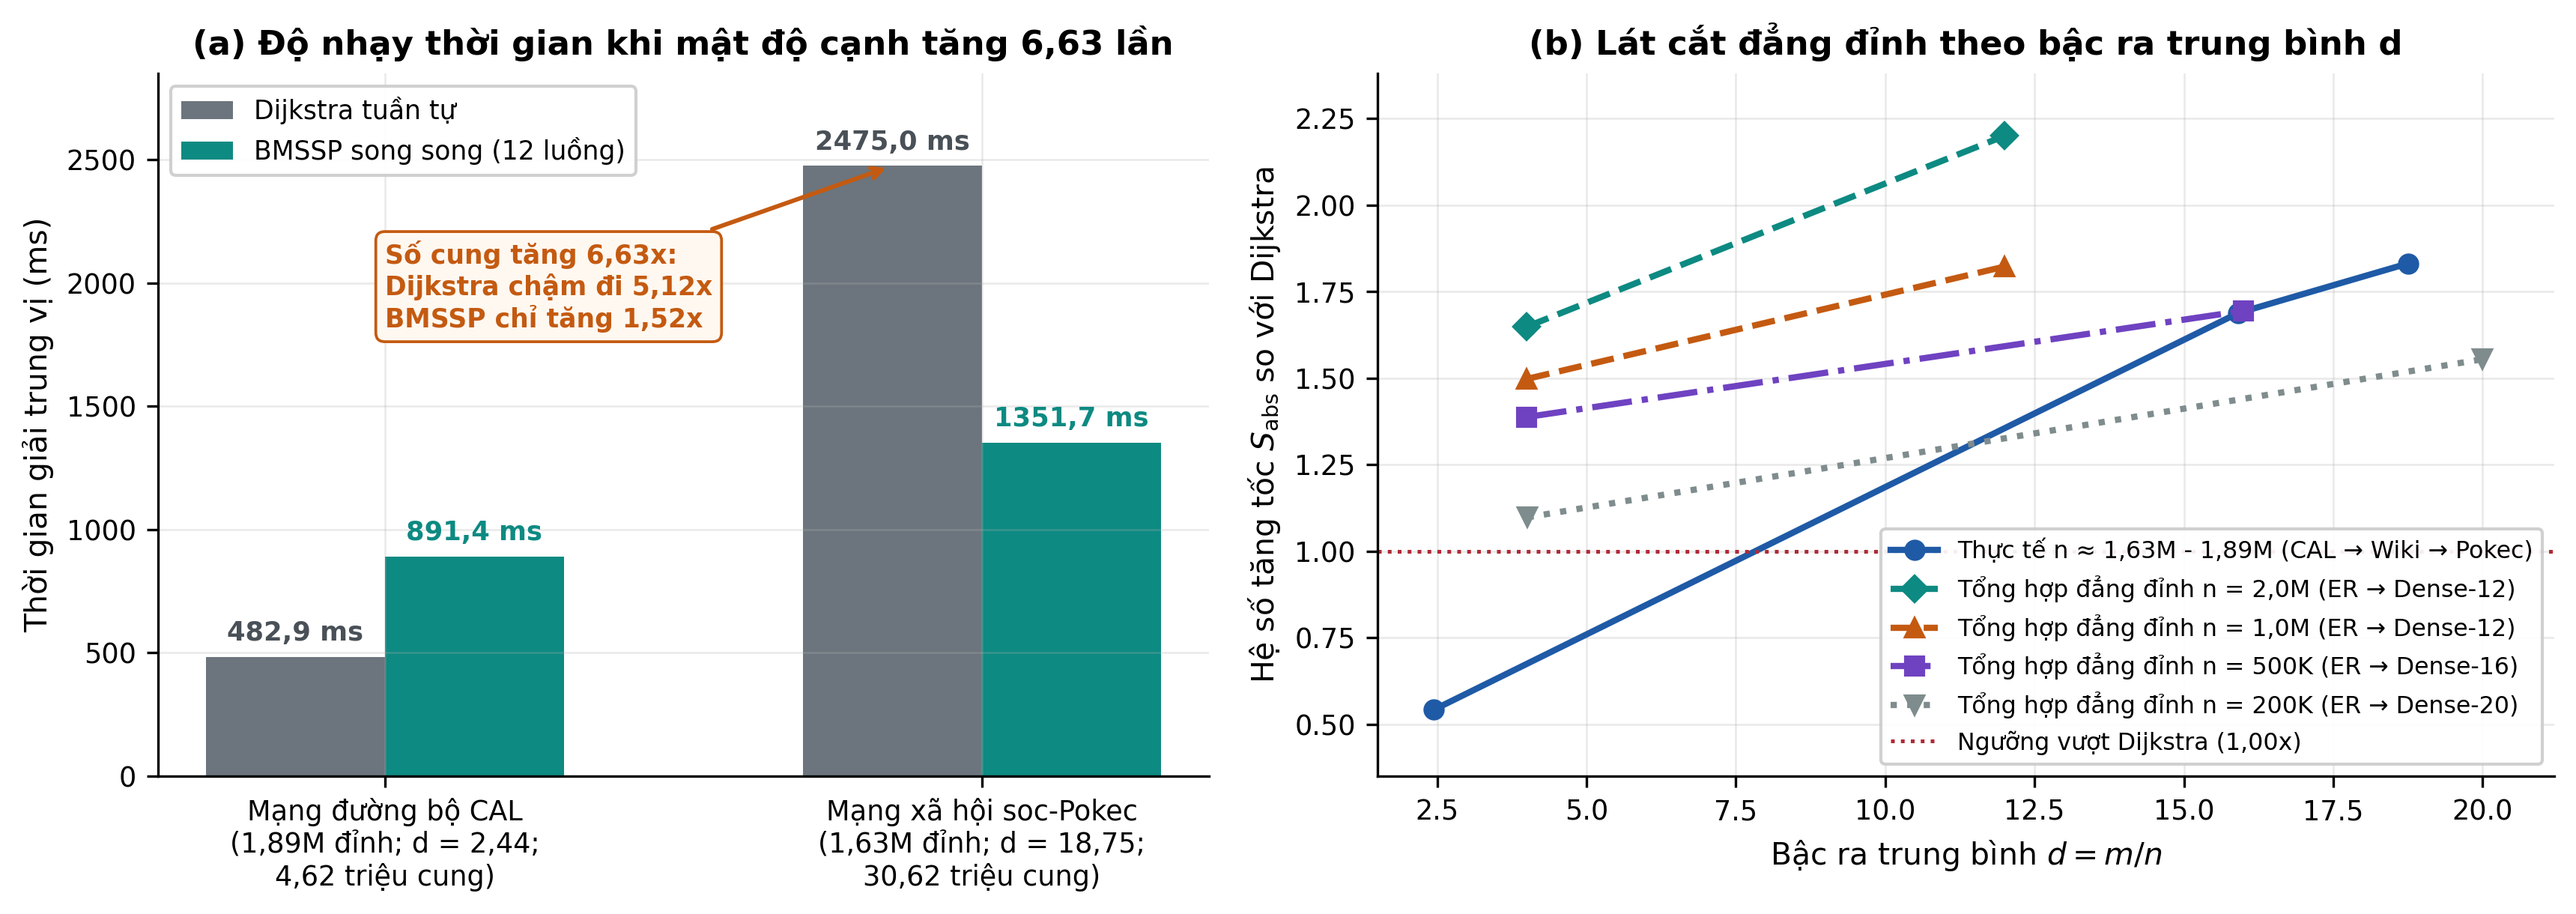
\includegraphics[width=0.96\linewidth]{image/ch3_degree_impact.png}
\caption{Độ nhạy thời gian đối lập khi mật độ cạnh tăng 6,63 lần từ mạng đường bộ \texttt{CAL} sang mạng xã hội \texttt{soc-Pokec} và các lát cắt đẳng đỉnh theo bậc trung bình $d$.}
\label{fig:degree_impact}
\end{figure}

Bằng chứng thực nghiệm rõ nét nhất thể hiện trên Hình~\ref{fig:degree_impact}a khi đối chiếu hai mạng thực tế có quy mô đỉnh tương đương khoảng $1{,}63\mathrm{M}$--$1{,}89\mathrm{M}$ là \texttt{CAL} và \texttt{soc-Pokec}: khi số cung tăng gấp $6{,}63$ lần từ $4{,}62$ triệu lên $30{,}62$ triệu cung, Dijkstra tuần tự bị chậm đi tới $5{,}12$ lần từ $482{,}93\,\mathrm{ms}$ lên $2\,474{,}98\,\mathrm{ms}$, trái lại hệ thống BMSSP ở $12$ luồng chỉ tăng thời gian đúng $1{,}52$ lần từ $891{,}43\,\mathrm{ms}$ lên $1\,351{,}73\,\mathrm{ms}$. Trên Hình~\ref{fig:degree_impact}b, mọi lát cắt giữ cố định quy mô đỉnh từ $200\mathrm{K}$ đến $2{,}0\mathrm{M}$ đều khẳng định quy luật nhất quán rằng bậc trung bình $d$ càng cao thì hệ số tăng tốc $S_{\mathrm{abs}}$ càng lớn.

\begin{figure}[!htb]
\centering
\resizebox{0.96\textwidth}{!}{%
\begin{tikzpicture}[>=latex, font=\scriptsize]
    % Biểu đồ thanh chồng ngang 100% (chiều dài thanh = 10.0 cm tương ứng 100%)
    \fill[orange!72!black] (0.0, 4.35) rectangle (0.45, 4.60);
    \node[anchor=west] at (0.55, 4.47) {Điều phối tuần tự $T_{\mathrm{seq}}(n)$};
    \fill[blue!55!black] (4.05, 4.35) rectangle (4.50, 4.60);
    \node[anchor=west] at (4.60, 4.47) {Quản lý và rút biên $\mathcal{D}$};
    \fill[teal!75!black] (7.65, 4.35) rectangle (8.10, 4.60);
    \node[anchor=west] at (8.20, 4.47) {Duyệt và thư giãn cạnh CSR song song};

    \foreach \v/\lbl in {0/0\%, 2.5/25\%, 5.0/50\%, 7.5/75\%, 10.0/100\%} {
        \draw[gray!25, thin] (\v, 0.30) -- (\v, 4.05);
        \draw[black!70] (\v, 0.30) -- (\v, 0.20);
        \node[anchor=north] at (\v, 0.16) {\lbl};
    }
    \draw[thick, black!80] (0, 0.30) -- (10.0, 0.30);

    % Hàng 1: Đồ thị nhỏ trong L3 (cit-HepPh) -> 48% + 34% + 18%
    \node[anchor=east, align=right, text width=3.4cm] at (-0.18, 3.62) {\textbf{Đồ thị nhỏ trong L3}\\(\texttt{cit-HepPh}; $34{,}5\mathrm{K}$)};
    \fill[orange!72!black] (0.00, 3.40) rectangle (4.80, 3.84); \node[text=white, font=\scriptsize\bfseries] at (2.40, 3.62) {48\%};
    \fill[blue!55!black]   (4.80, 3.40) rectangle (8.20, 3.84); \node[text=white, font=\scriptsize\bfseries] at (6.50, 3.62) {34\%};
    \fill[teal!75!black]   (8.20, 3.40) rectangle (10.00, 3.84); \node[text=white, font=\scriptsize\bfseries] at (9.10, 3.62) {18\%};

    % Hàng 2: Đường bộ biên hẹp (NW / CAL) -> 39% + 33% + 28%
    \node[anchor=east, align=right, text width=3.4cm] at (-0.18, 2.68) {\textbf{Đường bộ biên hẹp}\\(\texttt{NW}, \texttt{CAL}; $d \approx 2{,}4$)};
    \fill[orange!72!black] (0.00, 2.46) rectangle (3.90, 2.90); \node[text=white, font=\scriptsize\bfseries] at (1.95, 2.68) {39\%};
    \fill[blue!55!black]   (3.90, 2.46) rectangle (7.20, 2.90); \node[text=white, font=\scriptsize\bfseries] at (5.55, 2.68) {33\%};
    \fill[teal!75!black]   (7.20, 2.46) rectangle (10.00, 2.90); \node[text=white, font=\scriptsize\bfseries] at (8.60, 2.68) {28\%};

    % Hàng 3: Mạng Web điểm cắt (web-BerkStan) -> 22% + 31% + 47%
    \node[anchor=east, align=right, text width=3.4cm] at (-0.18, 1.74) {\textbf{Mạng Web điểm cắt}\\(\texttt{web-BerkStan}; $d = 11{,}1$)};
    \fill[orange!72!black] (0.00, 1.52) rectangle (2.20, 1.96); \node[text=white, font=\scriptsize\bfseries] at (1.10, 1.74) {22\%};
    \fill[blue!55!black]   (2.20, 1.52) rectangle (5.30, 1.96); \node[text=white, font=\scriptsize\bfseries] at (3.75, 1.74) {31\%};
    \fill[teal!75!black]   (5.30, 1.52) rectangle (10.00, 1.96); \node[text=white, font=\scriptsize\bfseries] at (7.65, 1.74) {47\%};

    % Hàng 4: Đồ thị lớn bậc cao (soc-Pokec / D12_2M) -> 12% + 24% + 64%
    \node[anchor=east, align=right, text width=3.4cm] at (-0.18, 0.80) {\textbf{Mạng lớn bậc cao}\\(\texttt{Pokec}, \texttt{D12\_2M}; $d \ge 12$)};
    \fill[orange!72!black] (0.00, 0.58) rectangle (1.20, 1.02); \node[text=white, font=\scriptsize\bfseries] at (0.60, 0.80) {12\%};
    \fill[blue!55!black]   (1.20, 0.58) rectangle (3.60, 1.02); \node[text=white, font=\scriptsize\bfseries] at (2.40, 0.80) {24\%};
    \fill[teal!75!black]   (3.60, 0.58) rectangle (10.00, 1.02); \node[text=white, font=\scriptsize\bfseries] at (6.80, 0.80) {64\%};
\end{tikzpicture}%
}
\caption{Sự dịch chuyển tỷ trọng thời gian giữa ba thành phần chi phí của Công thức~\eqref{eq:emp-bmssp} ở cấu hình 8--12 luồng qua bốn chế độ cấu trúc đồ thị.}
\label{fig:tikz_arch_regime}
\end{figure}

Sự dịch chuyển tỷ trọng của ba thành phần trong Công thức~\eqref{eq:emp-bmssp} được tổng kết trực quan trên Hình~\ref{fig:tikz_arch_regime}, qua đó chỉ rõ hai nút thắt còn giới hạn hệ số mở rộng tối đa của hệ thống. Thứ nhất, trên đồ thị nhỏ hoặc mạng đường bộ biên hẹp, phần lớn đợt duyệt rơi dưới ngưỡng $\Theta_{\mathrm{cutoff}}$ nên phần việc tuần tự $T_{\mathrm{seq}}(n)$ cùng thao tác \textsc{Pull} chiếm hơn $70\%$ tổng thời gian chạy. Thứ hai, khi chuyển sang mạng lớn bậc cao như \texttt{soc-Pokec} và \texttt{D12\_2M}, pha quét cạnh CSR song song mở rộng lên chiếm phần lớn khối lượng tính toán giúp thuật toán bứt tốc mạnh mẽ; tuy vậy, khoảng một phần ba thời gian còn lại vẫn nằm ở thao tác \textsc{Pull} tuần tự dưới khóa rút riêng kết hợp giới hạn băng thông bộ nhớ chia sẻ của $6$ lõi vật lý, giữ hệ số tự tăng tốc nội tại $S_{\mathrm{self}}$ bão hòa trong dải $1{,}84\times$--$2{,}28\times$.

\subsection{Quy luật mặt phẳng pha $(n, d)$ và miền lựa chọn thuật toán}\label{subsec:c3-phase-law}

Để tổng quát hóa định lượng kết quả trên toàn bộ $23$ bộ dữ liệu, nhóm tiến hành khớp mô hình hồi quy mặt phản ứng log-tuyến tính của hệ số tăng tốc tuyệt đối $S_{\mathrm{abs}}$ theo $\log_{10} n$, $\log_{10} d$ và đặc trưng hình học phẳng của mạng đường bộ. Như trình bày trên Hình~\ref{fig:phase_nd}b, mô hình thực nghiệm đạt hệ số xác định $R^2 = 0{,}9018$, giải thích hơn $90\%$ phương sai tốc độ quan sát được trên phần cứng thực tế.

\begin{figure}[!htb]
\centering
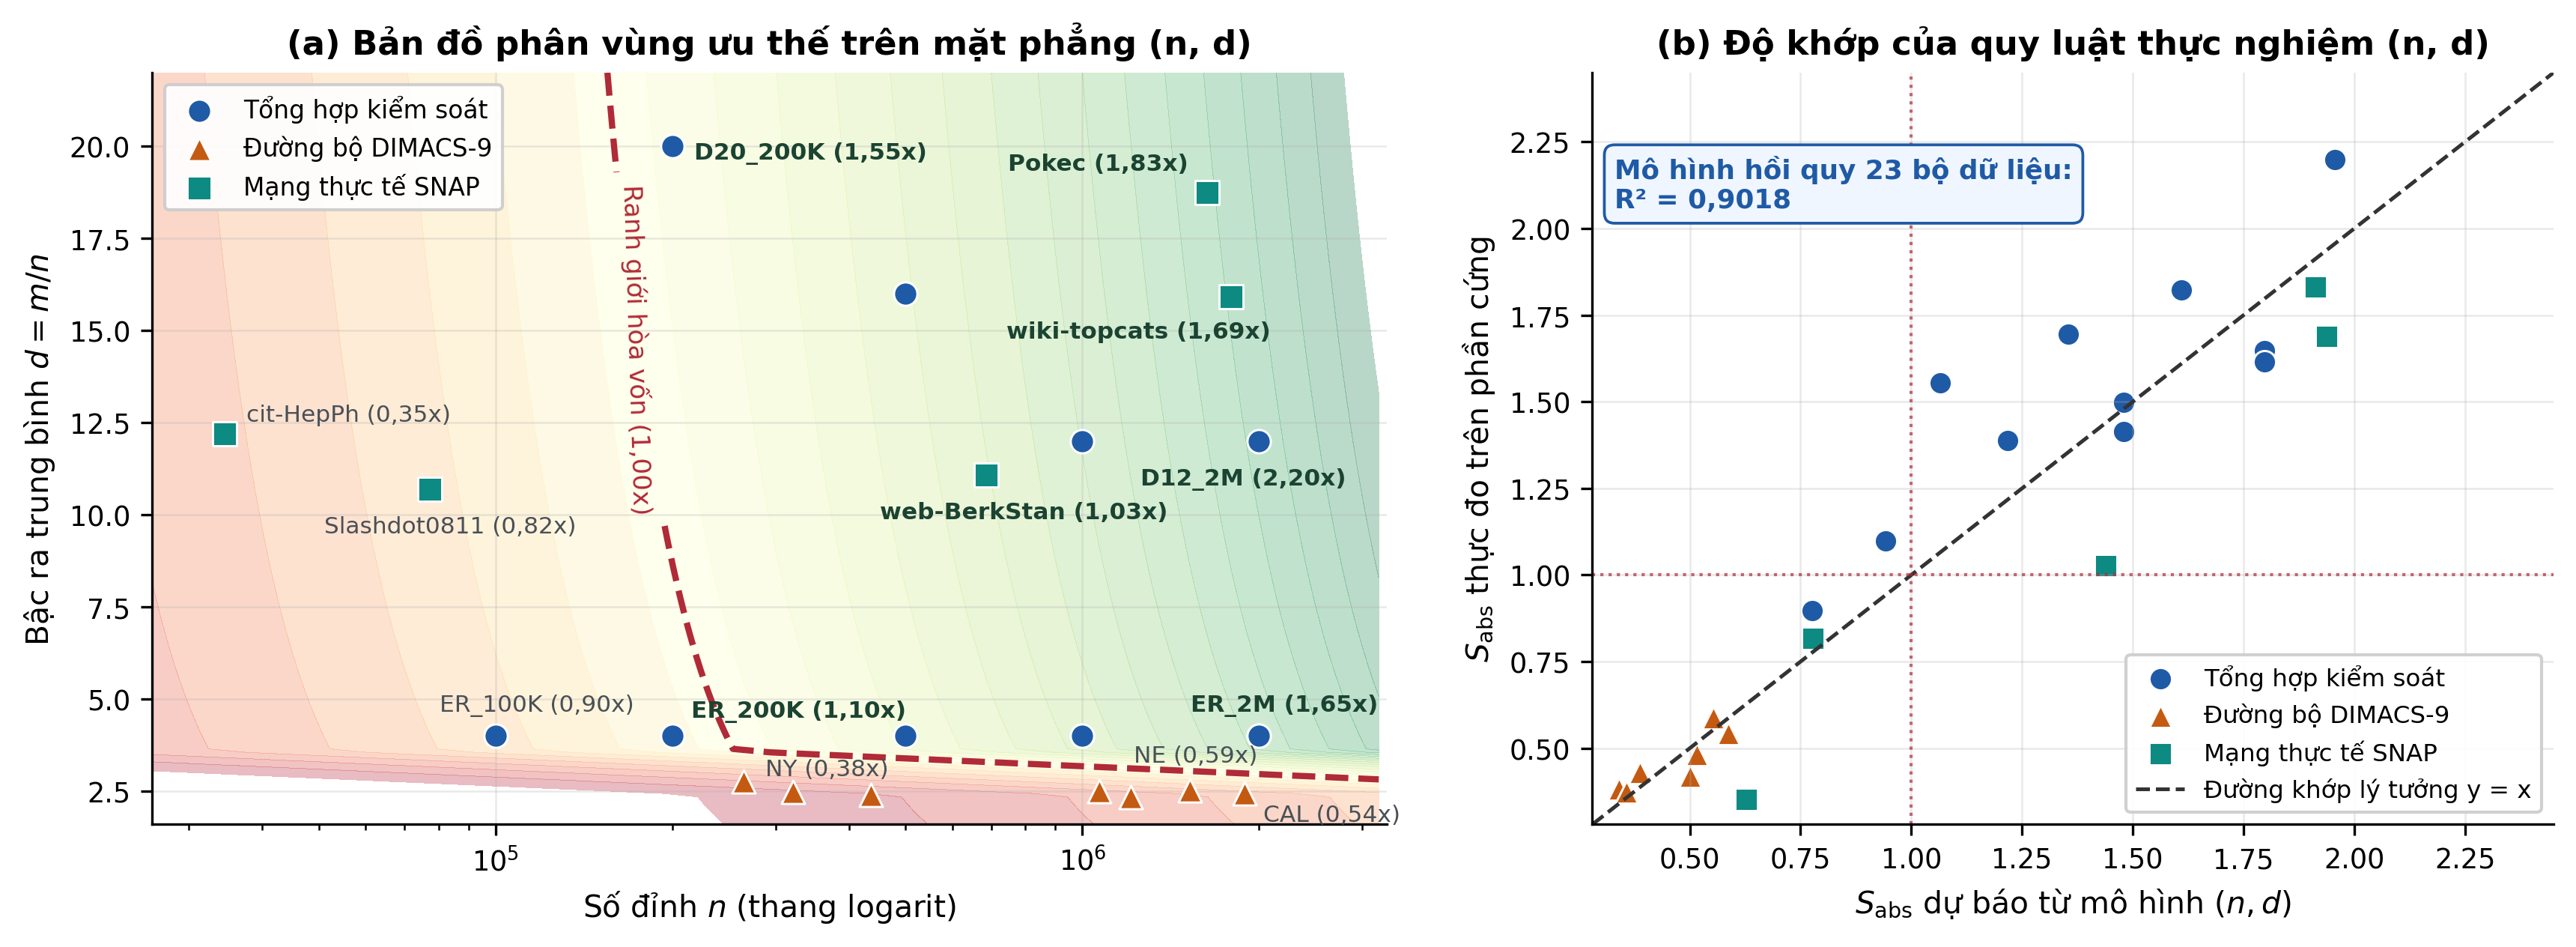
\includegraphics[width=0.96\linewidth]{image/ch3_phase_diagram_nd.png}
\caption{Bản đồ phân vùng ưu thế giữa Dijkstra tuần tự và BMSSP song song trên mặt phẳng $(n, d)$ cùng kiểm định độ khớp mô hình hồi quy trên 23 bộ dữ liệu thực nghiệm.}
\label{fig:phase_nd}
\end{figure}

Bản đồ pha trên Hình~\ref{fig:phase_nd}a phân tách không gian tham số $(n, d)$ qua đường ranh giới hòa vốn $S_{\mathrm{abs}} = 1{,}00\times$ thành hai miền ưu thế rõ rệt, được đúc kết thành quy tắc lựa chọn thực tiễn trong Bảng~\ref{tab:selection_guide}. Bên trái và phía dưới đường ranh giới là miền ưu thế của Dijkstra tuần tự, bao gồm mọi đồ thị quy mô nhỏ dưới $150\,000$ đỉnh nằm trọn trong bộ nhớ đệm và các mạng phẳng bậc cực thấp $d \le 3$ có mặt sóng mở rộng hẹp. Phía trên và bên phải đường ranh giới là miền ưu thế của BMSSP song song: trên đồ thị kết nối phân tán đều có $d \ge 4$, thuật toán vượt qua Dijkstra từ mốc $150\,000$--$200\,000$ đỉnh; trên các mạng thực tế có tính phân cụm cục bộ như Web và mạng xã hội với $d \ge 11$, điểm cắt nằm quanh mốc $450\,000$--$500\,000$ đỉnh tới được như trường hợp \texttt{web-BerkStan} và mở rộng ưu thế lên $1{,}69\times$--$2{,}20\times$ ở quy mô hàng triệu đỉnh.

\begin{table}[!htb]
\centering
{\small\setlength{\tabcolsep}{5pt}\setlength{\baselineskip}{13.5pt}
\begin{tabularx}{\textwidth}{@{} >{\raggedright\arraybackslash}p{3.65cm} >{\raggedright\arraybackslash}p{2.75cm} >{\raggedright\arraybackslash}X @{}}
\toprule
\textbf{Miền tham số $(n, d)$} & \textbf{Phương pháp ưu thế} & \textbf{Cơ sở kỹ thuật thực nghiệm} \\
\midrule
Đồ thị nhỏ $n < 150\,000$ ở mọi mức bậc $d$ & Dijkstra tuần tự & Dữ liệu nằm gọn trong bộ nhớ đệm L2 và L3, thời gian giải dưới $55\,\mathrm{ms}$ nên tránh được chi phí khởi tạo đệ quy và đồng bộ luồng. \\
\addlinespace[5pt]
Mạng phẳng hai chiều bậc rất thấp $d \le 3$ với $n \le 2\mathrm{M}$ & Dijkstra tuần tự & Mặt sóng địa lý hẹp thường xuyên rơi dưới ngưỡng $\Theta_{\mathrm{cutoff}} = 2048$, trong khi Dijkstra hưởng lợi mạnh từ tính cục bộ không gian. \\
\addlinespace[5pt]
Đồ thị trung bình $n \in [200\mathrm{K}, 700\mathrm{K}]$ có $d \ge 4$ ngẫu nhiên hoặc $d \ge 11$ thực tế & BMSSP song song $8$ luồng & Khối lượng cạnh mỗi lát đủ lớn để bù đắp chi phí điều phối, bắt đầu vượt Dijkstra với $S_{\mathrm{abs}}$ từ $1{,}03\times$ đến $1{,}69\times$. \\
\addlinespace[5pt]
Đồ thị quy mô lớn $n \ge 1\,000\,000$ có $d \ge 4$, đặc biệt mạng bậc cao $d \in [12, 20]$ & BMSSP song song $8\text{--}12$ luồng & Hàng đợi của Dijkstra tràn bộ nhớ đệm L3, còn BMSSP khai thác tốt quét CSR đa luồng, đạt $S_{\mathrm{abs}}$ từ $1{,}41\times$ đến $2{,}20\times$. \\
\bottomrule
\end{tabularx}
}
\caption{Tổng hợp miền lựa chọn thuật toán thực tiễn theo số đỉnh $n$, bậc trung bình $d$ và cấu trúc hình học đồ thị.}
\label{tab:selection_guide}
\end{table}

Cuối cùng, cần phân định trung thực về mặt học thuật rằng ưu thế tốc độ $1{,}41\times$--$2{,}20\times$ đạt được trên phần cứng thực tế là thành quả tổng hợp của việc song song hóa dữ liệu đa lõi trên kiến trúc lát khoảng cách kết hợp giảm thiểu tranh chấp trên \texttt{Concurrent\allowbreak FrontierD}, thay vì chỉ riêng cận tiệm cận tuần tự lý thuyết. Tại chế độ đơn luồng $p = 1$, cài đặt Dijkstra nhị phân vẫn nhanh hơn nhẹ từ $3\%$ đến $26\%$ trên các đồ thị lớn bậc cao nhờ cấu trúc mảng phẳng đơn giản; chính khả năng giải phóng song song hàng triệu phép thư giãn cạnh trong mỗi miền khoảng cách là yếu tố giúp BMSSP vượt lên rõ rệt trên các vi xử lý đa lõi hiện đại.

% ============================================================
% KẾT LUẬN
% ============================================================
\chapter*{KẾT LUẬN}
\addcontentsline{toc}{chapter}{Kết luận}

Tiểu luận đã nghiên cứu cơ sở lý thuyết, thiết kế kiến trúc hệ thống và triển khai hoàn chỉnh phiên bản song song của thuật toán \textit{Bounded Multi-Source Shortest Path} bằng ngôn ngữ C++20 kết hợp OpenMP cho bài toán đường đi ngắn nhất nguồn đơn trên đồ thị có hướng trọng số không âm. Bám sát mô hình đệ quy cắt lát khoảng cách của bài báo gốc, nhóm đã xây dựng kiến trúc phân bốn tầng tách biệt giao diện biên \texttt{IFrontierD} với tầng đồng bộ phần cứng, kết hợp bản ghi trạng thái đỉnh nguyên tử 128-bit tích hợp đường đọc nhanh 64-bit, cấu trúc biên hai phân vùng \texttt{Concurrent\allowbreak FrontierD} sử dụng danh sách nhảy khối kiểu B-Link có thu hồi bộ nhớ theo kỷ nguyên EBR, bể cấp phát khối cục bộ theo luồng và kỹ thuật chia tải cạnh dựa trên mảng tổng tiền tố bậc ra.

Tính đúng đắn của hệ thống được xác nhận độc lập trước khi đánh giá hiệu năng thông qua bốn bộ kiểm thử tự động chuyên sâu, bao gồm hơn $1{,}56$ triệu phép kiểm tra bất biến, bài đo chịu tải đồng thời $32$ luồng với mười triệu thao tác biên và $240$ lượt kiểm thử các trường hợp biên như chu trình trọng số $0$, đường đi gần hòa hay đỉnh siêu bậc. Trên toàn bộ $23$ bộ dữ liệu thực nghiệm trải rộng tới $2\,000\,000$ đỉnh và $30\,622\,564$ cung ở mọi cấu hình từ $1$ đến $12$ luồng, khoảng cách ngắn nhất tìm được đều trùng khớp tuyệt đối với bộ giải đối chứng Dijkstra tuần tự.

Về phương diện hiệu năng thực thi trên vi xử lý $6$ lõi $12$ luồng, nghiên cứu đã xác lập được mối liên hệ định lượng chặt chẽ với hệ số xác định $R^2 = 0{,}9018$ giữa quy mô đỉnh $n$, bậc trung bình $d = m/n$ và tốc độ tương đối của hai thuật toán. Thực nghiệm chỉ rõ trên đồ thị nhỏ dưới $150\,000$ đỉnh hoặc trên $7$ mạng giao thông đường bộ phẳng DIMACS-9 có bậc rất thấp $d \in [2{,}34;\, 2{,}76]$, mặt sóng mở rộng hẹp thường xuyên rơi dưới ngưỡng độ hạt $\Theta_{\mathrm{cutoff}} = 2048$ nên Dijkstra tuần tự vẫn giữ ưu thế tốc độ, dù tỷ số chênh lệch thu hẹp dần từ $2{,}67\times$ xuống $1{,}70\times$ khi quy mô vượt bộ nhớ đệm L3. Ngược lại, khi bậc đỉnh và quy mô tăng lên, hệ thống BMSSP song song chính thức vượt qua Dijkstra tại mốc \texttt{ER\_200K} trên dữ liệu tổng hợp và tại mạng liên kết Web \texttt{web-BerkStan} với $S_{\mathrm{abs}} = 1{,}03\times$ trên dữ liệu thực tế. Ở quy mô hàng triệu đỉnh và bậc trung bình từ $12$ đến $20$, hệ thống đạt hệ số tự tăng tốc nội tại $1{,}84\times$--$2{,}28\times$, giải nhanh hơn Dijkstra tuần tự từ $1{,}69\times$ trên \texttt{wiki-topcats}, $1{,}83\times$ trên mạng xã hội \texttt{soc-Pokec} cho đến $2{,}20\times$ trên đồ thị tổng hợp hai triệu đỉnh.

Bên cạnh những kết quả đạt được, hệ thống hiện tại vẫn tồn tại một số giới hạn kỹ thuật mở ra hướng phát triển tiếp theo. Trước hết, thao tác rút biên \textsc{Pull} và chèn tiền tố \textsc{BatchPrepend} vẫn thực thi tuần tự trên luồng điều phối nên tạo thành cận trên của đường găng khi số lõi vật lý tăng cao; việc nghiên cứu kỹ thuật rút biên và phân hoạch khối song song sẽ giúp nâng cao hơn nữa khả năng mở rộng đa luồng. Ngoài ra, các phép đo hiện mới thực hiện trên một vi xử lý máy trạm $6$ lõi vật lý với chế độ tắt biến đổi bậc hằng số mặc định; khảo sát hệ thống trên các máy chủ nhiều lõi vật lý có băng thông bộ nhớ lớn hơn, tự động thích ứng ngưỡng độ hạt $\Theta_{\mathrm{cutoff}}$ theo độ rộng mặt sóng thực tế hoặc kết hợp tăng tốc pha thư giãn cạnh mật độ cao trên GPU sẽ là những hướng mở rộng giàu tiềm năng trong tương lai.

% ============================================================
% TÀI LIỆU THAM KHẢO
% ============================================================
\newpage
\addcontentsline{toc}{chapter}{Tài liệu tham khảo}
\begin{thebibliography}{99}

\bibitem{duan2025breaking}
R. Duan, J. Mao, X. Mao, X. Shu, and L. Yin.
\textit{Breaking the Sorting Barrier for Directed Single-Source Shortest Paths.}
In Proceedings of the 57th Annual ACM Symposium on Theory of Computing (STOC '25), ACM, 2025.

\bibitem{dijkstra1959note}
E. W. Dijkstra.
\textit{A Note on Two Problems in Connexion with Graphs.}
Numerische Mathematik, 1(1):269--271, 1959.

\bibitem{bellman1958routing}
R. Bellman.
\textit{On a Routing Problem.}
Quarterly of Applied Mathematics, 16(1):87--90, 1958.

\bibitem{cormen2022introduction}
T. H. Cormen, C. E. Leiserson, R. L. Rivest, and C. Stein.
\textit{Introduction to Algorithms}, 4th edition.
The MIT Press, Cambridge, MA, 2022.

\bibitem{fredman1987fibonacci}
M. L. Fredman and R. E. Tarjan.
\textit{Fibonacci Heaps and Their Uses in Improved Network Optimization Algorithms.}
Journal of the ACM, 34(3):596--615, 1987.

\bibitem{haeupler2024universal}
B. Haeupler, R. Hlad{\'\i}k, V. Rozho{\v{n}}, R. E. Tarjan, and J. T{\v{e}}tek.
\textit{Universal Optimality of Dijkstra via Beyond-Worst-Case Heaps.}
In Proceedings of the 65th Annual IEEE Symposium on Foundations of Computer Science (FOCS), 2024.

\bibitem{frederickson1983data}
G. N. Frederickson.
\textit{Data Structures for On-Line Updating of Minimum Spanning Trees.}
In Proceedings of the 15th Annual ACM Symposium on Theory of Computing (STOC), pp. 252--257, 1983.

\bibitem{meyer2003deltastepping}
U. Meyer and P. Sanders.
\textit{$\Delta$-stepping: A Parallelizable Shortest Path Algorithm.}
Journal of Algorithms, 49(1):114--152, 2003.

\bibitem{brent1974parallel}
R. P. Brent.
\textit{The Parallel Evaluation of General Arithmetic Expressions.}
Journal of the ACM, 21(2):201--206, 1974.

\bibitem{amdahl1967validity}
G. M. Amdahl.
\textit{Validity of the Single Processor Approach to Achieving Large Scale Computing Capabilities.}
In Proceedings of the AFIPS Spring Joint Computer Conference, pp. 483--485, 1967.

\bibitem{dagum1998openmp}
L. Dagum and R. Menon.
\textit{OpenMP: An Industry-Standard API for Shared-Memory Programming.}
IEEE Computational Science and Engineering, 5(1):46--55, 1998.

\bibitem{openmp52}
OpenMP Architecture Review Board.
\textit{OpenMP Application Programming Interface, Version 5.2.}
November 2021. \url{https://www.openmp.org/specifications/}

\bibitem{saad2003iterative}
Y. Saad.
\textit{Iterative Methods for Sparse Linear Systems}, 2nd edition.
Society for Industrial and Applied Mathematics (SIAM), 2003.

\bibitem{shun2013ligra}
J. Shun and G. E. Blelloch.
\textit{Ligra: A Lightweight Graph Processing Framework for Shared Memory.}
In Proceedings of the 18th ACM SIGPLAN Symposium on Principles and Practice of Parallel Programming (PPoPP '13), pp. 135--146, 2013.

\bibitem{herlihy2012art}
M. Herlihy and N. Shavit.
\textit{The Art of Multiprocessor Programming}, Revised 1st edition.
Morgan Kaufmann, 2012.

\bibitem{intel2023sdm}
Intel Corporation.
\textit{Intel\textsuperscript{\textregistered} 64 and IA-32 Architectures Software Developer's Manual, Volume 2: Instruction Set Reference.}
2023.

\bibitem{berger2000hoard}
E. D. Berger, K. S. McKinley, R. D. Blumofe, and P. R. Wilson.
\textit{Hoard: A Scalable Memory Allocator for Multithreaded Applications.}
In Proceedings of the 9th International Conference on Architectural Support for Programming Languages and Operating Systems (ASPLOS IX), pp. 117--128, 2000.

\bibitem{blelloch1990prefix}
G. E. Blelloch.
\textit{Prefix Sums and Their Applications.}
Technical Report CMU-CS-90-190, School of Computer Science, Carnegie Mellon University, 1990.

\bibitem{tsigas2003parallel}
P. Tsigas and Y. Zhang.
\textit{A Simple, Fast Parallel Implementation of Quicksort and its Performance Evaluation on SUN Enterprise 10000.}
In Proceedings of the 11th Euromicro Conference on Parallel, Distributed and Network-Based Processing (PDP '03), pp. 372--381, 2003.

\bibitem{serebryany2009threadsanitizer}
K. Serebryany and T. Iskhodzhanov.
\textit{ThreadSanitizer -- Data Race Detection in Practice.}
In Proceedings of the Workshop on Binary Instrumentation and Applications (WBIA '09), pp. 62--71, 2009.

\bibitem{pugh1990skip}
W. Pugh.
\textit{Skip Lists: A Probabilistic Alternative to Balanced Trees.}
Communications of the ACM, 33(6):668--676, 1990.

\bibitem{lehman1981efficient}
P. L. Lehman and S. B. Yao.
\textit{Efficient Locking for Concurrent Operations on B-Trees.}
ACM Transactions on Database Systems (TODS), 6(4):650--670, 1981.

\bibitem{demetrescu2009dimacs}
C. Demetrescu, A. V. Goldberg, and D. S. Johnson.
\textit{The Shortest Path Problem: Ninth DIMACS Implementation Challenge.}
DIMACS Book Series, Vol. 74, American Mathematical Society, 2009.

\bibitem{leskovec2014snap}
J. Leskovec and A. Krevl.
\textit{SNAP Datasets: Stanford Large Network Dataset Collection.}
June 2014. \url{http://snap.stanford.edu/data}

\end{thebibliography}
